\documentclass[]{article}
\usepackage{lmodern}
\usepackage{amssymb,amsmath}
\usepackage{ifxetex,ifluatex}
\usepackage{fixltx2e} % provides \textsubscript
\ifnum 0\ifxetex 1\fi\ifluatex 1\fi=0 % if pdftex
  \usepackage[T1]{fontenc}
  \usepackage[utf8]{inputenc}
\else % if luatex or xelatex
  \ifxetex
    \usepackage{mathspec}
    \usepackage{xltxtra,xunicode}
  \else
    \usepackage{fontspec}
  \fi
  \defaultfontfeatures{Mapping=tex-text,Scale=MatchLowercase}
  \newcommand{\euro}{€}
\fi
% use upquote if available, for straight quotes in verbatim environments
\IfFileExists{upquote.sty}{\usepackage{upquote}}{}
% use microtype if available
\IfFileExists{microtype.sty}{\usepackage{microtype}}{}
\usepackage[margin=1in]{geometry}
\usepackage{color}
\usepackage{fancyvrb}
\newcommand{\VerbBar}{|}
\newcommand{\VERB}{\Verb[commandchars=\\\{\}]}
\DefineVerbatimEnvironment{Highlighting}{Verbatim}{commandchars=\\\{\}}
% Add ',fontsize=\small' for more characters per line
\newenvironment{Shaded}{}{}
\newcommand{\AlertTok}[1]{\textcolor[rgb]{1.00,0.00,0.00}{\textbf{#1}}}
\newcommand{\AnnotationTok}[1]{\textcolor[rgb]{0.38,0.63,0.69}{\textbf{\textit{#1}}}}
\newcommand{\AttributeTok}[1]{\textcolor[rgb]{0.49,0.56,0.16}{#1}}
\newcommand{\BaseNTok}[1]{\textcolor[rgb]{0.25,0.63,0.44}{#1}}
\newcommand{\BuiltInTok}[1]{#1}
\newcommand{\CharTok}[1]{\textcolor[rgb]{0.25,0.44,0.63}{#1}}
\newcommand{\CommentTok}[1]{\textcolor[rgb]{0.38,0.63,0.69}{\textit{#1}}}
\newcommand{\CommentVarTok}[1]{\textcolor[rgb]{0.38,0.63,0.69}{\textbf{\textit{#1}}}}
\newcommand{\ConstantTok}[1]{\textcolor[rgb]{0.53,0.00,0.00}{#1}}
\newcommand{\ControlFlowTok}[1]{\textcolor[rgb]{0.00,0.44,0.13}{\textbf{#1}}}
\newcommand{\DataTypeTok}[1]{\textcolor[rgb]{0.56,0.13,0.00}{#1}}
\newcommand{\DecValTok}[1]{\textcolor[rgb]{0.25,0.63,0.44}{#1}}
\newcommand{\DocumentationTok}[1]{\textcolor[rgb]{0.73,0.13,0.13}{\textit{#1}}}
\newcommand{\ErrorTok}[1]{\textcolor[rgb]{1.00,0.00,0.00}{\textbf{#1}}}
\newcommand{\ExtensionTok}[1]{#1}
\newcommand{\FloatTok}[1]{\textcolor[rgb]{0.25,0.63,0.44}{#1}}
\newcommand{\FunctionTok}[1]{\textcolor[rgb]{0.02,0.16,0.49}{#1}}
\newcommand{\ImportTok}[1]{#1}
\newcommand{\InformationTok}[1]{\textcolor[rgb]{0.38,0.63,0.69}{\textbf{\textit{#1}}}}
\newcommand{\KeywordTok}[1]{\textcolor[rgb]{0.00,0.44,0.13}{\textbf{#1}}}
\newcommand{\NormalTok}[1]{#1}
\newcommand{\OperatorTok}[1]{\textcolor[rgb]{0.40,0.40,0.40}{#1}}
\newcommand{\OtherTok}[1]{\textcolor[rgb]{0.00,0.44,0.13}{#1}}
\newcommand{\PreprocessorTok}[1]{\textcolor[rgb]{0.74,0.48,0.00}{#1}}
\newcommand{\RegionMarkerTok}[1]{#1}
\newcommand{\SpecialCharTok}[1]{\textcolor[rgb]{0.25,0.44,0.63}{#1}}
\newcommand{\SpecialStringTok}[1]{\textcolor[rgb]{0.73,0.40,0.53}{#1}}
\newcommand{\StringTok}[1]{\textcolor[rgb]{0.25,0.44,0.63}{#1}}
\newcommand{\VariableTok}[1]{\textcolor[rgb]{0.10,0.09,0.49}{#1}}
\newcommand{\VerbatimStringTok}[1]{\textcolor[rgb]{0.25,0.44,0.63}{#1}}
\newcommand{\WarningTok}[1]{\textcolor[rgb]{0.38,0.63,0.69}{\textbf{\textit{#1}}}}
\usepackage{graphicx}
\makeatletter
\def\maxwidth{\ifdim\Gin@nat@width>\linewidth\linewidth\else\Gin@nat@width\fi}
\def\maxheight{\ifdim\Gin@nat@height>\textheight\textheight\else\Gin@nat@height\fi}
\makeatother
% Scale images if necessary, so that they will not overflow the page
% margins by default, and it is still possible to overwrite the defaults
% using explicit options in \includegraphics[width, height, ...]{}
\setkeys{Gin}{width=\maxwidth,height=\maxheight,keepaspectratio}
\ifxetex
  \usepackage[setpagesize=false, % page size defined by xetex
              unicode=false, % unicode breaks when used with xetex
              xetex]{hyperref}
\else
  \usepackage[unicode=true]{hyperref}
\fi
\hypersetup{breaklinks=true,
            bookmarks=true,
            pdfauthor={Justin Le},
            pdftitle={Lenses embody Products, Prisms embody Sums},
            colorlinks=true,
            citecolor=blue,
            urlcolor=blue,
            linkcolor=magenta,
            pdfborder={0 0 0}}
\urlstyle{same}  % don't use monospace font for urls
% Make links footnotes instead of hotlinks:
\renewcommand{\href}[2]{#2\footnote{\url{#1}}}
\setlength{\parindent}{0pt}
\setlength{\parskip}{6pt plus 2pt minus 1pt}
\setlength{\emergencystretch}{3em}  % prevent overfull lines
\setcounter{secnumdepth}{0}

\title{Lenses embody Products, Prisms embody Sums}
\author{Justin Le}
\date{June 11, 2018}

\begin{document}
\maketitle

\emph{Originally posted on
\textbf{\href{https://blog.jle.im/entry/lenses-products-prisms-sums.html}{in
Code}}.}

I've written about a variety of topics on this blog, but one thing I haven't
touched in too much detail is the topic of lenses and optics. A big part of this
is because there are already so many great resources on lenses.

This post won't be a ``lens tutorial'', but rather a dive into an perspective on
lenses and prisms that I've heard repeated many times (usually credited to
Edward Kmett, but shachaf has helped me trace the origins back to
\href{https://lpaste.net/77766}{this paste} by Reid Barton) but never quite
expanded on in-depth. In particular, I'm going to talk about the perspective of
lenses and prisms as embodying the essences of products and sums (respectively),
the insights that perspective brings, how well it flows into the ``profunctor
optics'' formulation, and how you can apply these observations to practical
usage of lenses and prisms.

The ``final code'' in this post is
\href{https://github.com/mstksg/inCode/tree/master/code-samples/misc/lenses-and-prisms.hs}{available
online} as a ``stack executable'' that, when run, will pop you into a
\emph{ghci} session with all of the final definitions in scope, so you can play
around with them :)

\hypertarget{an-algebraic-recap}{%
\section{An Algebraic Recap}\label{an-algebraic-recap}}

In Haskell, ``products and sums'' can roughly be said to correspond to ``tuples
and \texttt{Either}''. If I have two types \texttt{A} and \texttt{B},
\texttt{(A,\ B)} is their ``product'' type. It's often called an ``anonymous
product'', because we can make one without having to give it a fancy name. It's
called a product type because if \texttt{A} has
\includegraphics{https://latex.codecogs.com/png.latex?n} possible values and
\texttt{B} has \includegraphics{https://latex.codecogs.com/png.latex?m} possible
values, then \texttt{(A,\ B)} has
\includegraphics{https://latex.codecogs.com/png.latex?n\%20\%5Ctimes\%20m}
possible values\footnote{All of this is disregarding the notorious ``bottom''
  value that inhabits every type.}. And, \texttt{Either\ A\ B} is their
(anonymous) ``sum'' type. It's called a sum type because \texttt{Either\ A\ B}
has \includegraphics{https://latex.codecogs.com/png.latex?n\%20\%2B\%20m}
possible values. I won't go much deeper into this, but there are
\href{https://codewords.recurse.com/issues/three/algebra-and-calculus-of-algebraic-data-types}{many
useful summaries already online} on this topic!

\hypertarget{lets-get-productive}{%
\section{Let's Get Productive!}\label{lets-get-productive}}

It's easy to recognize \texttt{(Int,\ Bool)} as a product between \texttt{Int}
and \texttt{Bool}. However, did you know that some types are secretly product
types in disguise?

For example, here's a classic example of a data type often used with
\emph{lens}:

\begin{Shaded}
\begin{Highlighting}[]
\CommentTok{{-}{-} source: https://github.com/mstksg/inCode/tree/master/code{-}samples/misc/lenses{-}and{-}prisms.hs\#L145{-}L148}

\KeywordTok{data} \DataTypeTok{Person} \OtherTok{=} \DataTypeTok{P}
\NormalTok{    \{}\OtherTok{ \_pName ::} \DataTypeTok{String}
\NormalTok{    ,}\OtherTok{ \_pAge  ::} \DataTypeTok{Int}
\NormalTok{    \}}
\end{Highlighting}
\end{Shaded}

\texttt{Person} is an algebraic data type --- so-called because it is actually a
\emph{product} between a \texttt{String} and \texttt{Int}. \texttt{Person} is
\emph{isomorphic} to \texttt{(String,\ Int)}. I will be writing this as
\texttt{Person\ \textless{}\textasciitilde{}\textgreater{}\ (String,\ Int)}.

By \emph{isomorphic}, I mean that there are functions
\texttt{split\ ::\ Person\ -\textgreater{}\ (String,\ Int)} and
\texttt{unsplit\ ::\ (String,\ Int)\ -\textgreater{}\ Person} where
\texttt{unsplit\ .\ split\ =\ id} and \texttt{split\ .\ unsplit\ =\ id}. You can
think of this property as stating formally that you should be able to go from
one type to the other without ``losing any information''. Every single item in
one type gets paired to a specific item in the other, and vice versa, and
neither type is ``too big'' or ``too small''.

In our case, we have:

\begin{Shaded}
\begin{Highlighting}[]
\OtherTok{split ::} \DataTypeTok{Person} \OtherTok{{-}>}\NormalTok{ (}\DataTypeTok{String}\NormalTok{, }\DataTypeTok{Int}\NormalTok{)}
\NormalTok{split (}\DataTypeTok{P}\NormalTok{ n a) }\OtherTok{=}\NormalTok{ (n, a)}

\OtherTok{unsplit ::}\NormalTok{ (}\DataTypeTok{String}\NormalTok{, }\DataTypeTok{Int}\NormalTok{) }\OtherTok{{-}>} \DataTypeTok{Person}
\NormalTok{unsplit (n, a) }\OtherTok{=} \DataTypeTok{P}\NormalTok{ n a}
\end{Highlighting}
\end{Shaded}

And we can verify that \texttt{unsplit\ .\ split} is \texttt{id}:

\begin{Shaded}
\begin{Highlighting}[]
\NormalTok{unsplit }\OperatorTok{.}\OtherTok{ split ::} \DataTypeTok{Person} \OtherTok{{-}>} \DataTypeTok{Person}
\NormalTok{unsplit }\OperatorTok{.}\NormalTok{ split}
    \OtherTok{=}\NormalTok{ \textbackslash{}x          }\OtherTok{{-}>}\NormalTok{ unsplit (split x)        }\CommentTok{{-}{-} substitute definition of (.)}
    \OtherTok{=}\NormalTok{ \textbackslash{}}\KeywordTok{case} \DataTypeTok{P}\NormalTok{ n a }\OtherTok{{-}>}\NormalTok{ unsplit (split (}\DataTypeTok{P}\NormalTok{ n a))  }\CommentTok{{-}{-} expand patterns}
    \OtherTok{=}\NormalTok{ \textbackslash{}}\KeywordTok{case} \DataTypeTok{P}\NormalTok{ n a }\OtherTok{{-}>}\NormalTok{ unsplit (n, a)           }\CommentTok{{-}{-} substitute definition of split}
    \OtherTok{=}\NormalTok{ \textbackslash{}}\KeywordTok{case} \DataTypeTok{P}\NormalTok{ n a }\OtherTok{{-}>} \DataTypeTok{P}\NormalTok{ n a                    }\CommentTok{{-}{-} substitute definition of unsplit}
    \OtherTok{=}\NormalTok{ \textbackslash{}x      }\OtherTok{{-}>}\NormalTok{ x                            }\CommentTok{{-}{-} condense patterns}
    \OtherTok{=} \FunctionTok{id}                                      \CommentTok{{-}{-} definition of id}
\end{Highlighting}
\end{Shaded}

And verification of \texttt{split\ .\ unsplit\ =\ id} is left as an exercise.

There are some other interesting products in Haskell, too. One such example is
\texttt{NonEmpty\ a} (the type of a non-empty list) being a product between
\texttt{a} (the head/first item) and \texttt{{[}a{]}} (the tail/rest of the
items). This means that \texttt{NonEmpty\ a} is isomorphic to
\texttt{(a,\ {[}a{]})} --- we have
\texttt{NonEmpty\ a\ \textless{}\textasciitilde{}\textgreater{}\ (a,\ {[}a{]})}!
This is witnessed by functions
\texttt{split\ ::\ NonEmpty\ a\ -\textgreater{}\ (a,\ {[}a{]})} and
\texttt{unsplit\ ::\ (a,\ {[}a{]})\ -\textgreater{}\ NonEmpty\ a} where
\texttt{unsplit\ .\ split\ =\ id} and \texttt{split\ .\ unsplit\ =\ id}. See if
you can write these!

Another curious product is the fact that every type \texttt{a} is a product
between \emph{itself} and unit, \texttt{()}. Every type \texttt{a} is isomorphic
to \texttt{(a,\ ())} (which follows from the algebraic property
\includegraphics{https://latex.codecogs.com/png.latex?x\%20\%2A\%201\%20\%3D\%20x}).
Freaky, right?

\begin{Shaded}
\begin{Highlighting}[]
\CommentTok{{-}{-} a <\textasciitilde{}> (a, ())}

\OtherTok{split ::}\NormalTok{ a }\OtherTok{{-}>}\NormalTok{ (a, ())}
\NormalTok{split x }\OtherTok{=}\NormalTok{ (x, ())}

\OtherTok{unsplit ::}\NormalTok{ (a, ()) }\OtherTok{{-}>}\NormalTok{ a}
\NormalTok{unsplit (x, \_) }\OtherTok{=}\NormalTok{ x}
\end{Highlighting}
\end{Shaded}

One final interesting ``product in disguise'' is \texttt{Either\ a\ a}. ``But
wait,'' you say. ``That's a sum\ldots right??''

Well, yeah. But in addition, any \texttt{Either\ a\ a} is the product between
\texttt{Bool} and \texttt{a}. We can say that \texttt{Either\ a\ a} is
isomorphic to \texttt{(Bool,\ a)}! The \texttt{Bool} tells you ``left or
right?'' and the \texttt{a} is the contents:

\begin{Shaded}
\begin{Highlighting}[]
\CommentTok{{-}{-} Either a a <\textasciitilde{}> (Bool, a)}

\OtherTok{split ::} \DataTypeTok{Either}\NormalTok{ a a }\OtherTok{{-}>}\NormalTok{ (}\DataTypeTok{Bool}\NormalTok{, a)}
\NormalTok{split (}\DataTypeTok{Left}\NormalTok{  x) }\OtherTok{=}\NormalTok{ (}\DataTypeTok{False}\NormalTok{, x)}
\NormalTok{split (}\DataTypeTok{Right}\NormalTok{ x) }\OtherTok{=}\NormalTok{ (}\DataTypeTok{True}\NormalTok{ , x)}

\OtherTok{unsplit ::}\NormalTok{ (}\DataTypeTok{Bool}\NormalTok{, a) }\OtherTok{{-}>} \DataTypeTok{Either}\NormalTok{ a a}
\NormalTok{unsplit (}\DataTypeTok{False}\NormalTok{, x) }\OtherTok{=} \DataTypeTok{Left}\NormalTok{  x}
\NormalTok{unsplit (}\DataTypeTok{True}\NormalTok{ , x) }\OtherTok{=} \DataTypeTok{Right}\NormalTok{ x}
\end{Highlighting}
\end{Shaded}

Proving that \texttt{unsplit\ .\ split\ =\ id}:

\begin{Shaded}
\begin{Highlighting}[]
\NormalTok{unsplit }\OperatorTok{.}\OtherTok{ split ::} \DataTypeTok{Either}\NormalTok{ a a }\OtherTok{{-}>} \DataTypeTok{Either}\NormalTok{ a a}
\NormalTok{unsplit }\OperatorTok{.}\NormalTok{ split }\OtherTok{=}
    \OtherTok{=}\NormalTok{ \textbackslash{}x            }\OtherTok{{-}>}\NormalTok{ unsplit (split x)          }\CommentTok{{-}{-} substitute definition of (.)}
      \CommentTok{{-}{-} trying case 1}
    \OtherTok{=}\NormalTok{ \textbackslash{}}\KeywordTok{case} \DataTypeTok{Left}\NormalTok{  y }\OtherTok{{-}>}\NormalTok{ unsplit (split (}\DataTypeTok{Left}\NormalTok{  y))  }\CommentTok{{-}{-} expand pattern for case 1}
    \OtherTok{=}\NormalTok{ \textbackslash{}}\KeywordTok{case} \DataTypeTok{Left}\NormalTok{  y }\OtherTok{{-}>}\NormalTok{ unsplit (}\DataTypeTok{False}\NormalTok{, y)         }\CommentTok{{-}{-} substitute definition of split}
    \OtherTok{=}\NormalTok{ \textbackslash{}}\KeywordTok{case} \DataTypeTok{Left}\NormalTok{  y }\OtherTok{{-}>} \DataTypeTok{Left}\NormalTok{  y                    }\CommentTok{{-}{-} substitute definition of unsplit}
    \OtherTok{=}\NormalTok{ \textbackslash{}x            }\OtherTok{{-}>}\NormalTok{ x                          }\CommentTok{{-}{-} condense pattern for case 1}
    \OtherTok{=} \FunctionTok{id}                                          \CommentTok{{-}{-} definition of id}
      \CommentTok{{-}{-} trying case 2}
    \OtherTok{=}\NormalTok{ \textbackslash{}}\KeywordTok{case} \DataTypeTok{Right}\NormalTok{ y }\OtherTok{{-}>}\NormalTok{ unsplit (split (}\DataTypeTok{Right}\NormalTok{ y))  }\CommentTok{{-}{-} expand pattern for case 2}
    \OtherTok{=}\NormalTok{ \textbackslash{}}\KeywordTok{case} \DataTypeTok{Right}\NormalTok{ y }\OtherTok{{-}>}\NormalTok{ unsplit (}\DataTypeTok{True}\NormalTok{ , y)         }\CommentTok{{-}{-} substitute definition of split}
    \OtherTok{=}\NormalTok{ \textbackslash{}}\KeywordTok{case} \DataTypeTok{Right}\NormalTok{ y }\OtherTok{{-}>} \DataTypeTok{Right}\NormalTok{ y                    }\CommentTok{{-}{-} substitute definition of unsplit}
    \OtherTok{=}\NormalTok{ \textbackslash{}x            }\OtherTok{{-}>}\NormalTok{ x                          }\CommentTok{{-}{-} condense pattern for case 2}
    \OtherTok{=} \FunctionTok{id}                                          \CommentTok{{-}{-} definition of id}
\end{Highlighting}
\end{Shaded}

And \texttt{split\ .\ unsplit\ =\ id} is again left as an exercise.

(\texttt{\textbackslash{}case} here is from the \emph{-XLambdaCase} extension)

\hypertarget{lenses}{%
\subsection{Lenses}\label{lenses}}

So, how do lenses come into the picture?

Let's review a bit. A \texttt{Lens\textquotesingle{}\ s\ a} is a way to
``access'' an \texttt{a} ``inside'' an \texttt{s}, \emph{respecting some laws}.

A \texttt{Lens\textquotesingle{}\ s\ a} is a data type with the following API:

\begin{Shaded}
\begin{Highlighting}[]
\OtherTok{view ::} \DataTypeTok{Lens\textquotesingle{}}\NormalTok{ s a }\OtherTok{{-}>}\NormalTok{ (s }\OtherTok{{-}>}\NormalTok{ a)                }\CommentTok{{-}{-} get the \textquotesingle{}a\textquotesingle{} from an \textquotesingle{}s\textquotesingle{}}
\OtherTok{set  ::} \DataTypeTok{Lens\textquotesingle{}}\NormalTok{ s a }\OtherTok{{-}>}\NormalTok{ (a }\OtherTok{{-}>}\NormalTok{ s }\OtherTok{{-}>}\NormalTok{ s)           }\CommentTok{{-}{-} set the \textquotesingle{}a\textquotesingle{} inside an \textquotesingle{}s\textquotesingle{}}
\end{Highlighting}
\end{Shaded}

respecting
\href{https://www.schoolofhaskell.com/school/to-infinity-and-beyond/pick-of-the-week/a-little-lens-starter-tutorial\#the-lens-laws-}{the
lens laws} --- get-put, put-get, and put-put. Abstract mathematical laws are
great and all, but I'm going to tell you a secret that subsumes those laws.

At first, you might naively implement lenses like:

\begin{Shaded}
\begin{Highlighting}[]
\KeywordTok{data} \DataTypeTok{Lens\textquotesingle{}}\NormalTok{ s a }\OtherTok{=} \DataTypeTok{Lens\textquotesingle{}}
\NormalTok{    \{}\OtherTok{ view ::}\NormalTok{ s }\OtherTok{{-}>}\NormalTok{ a}
\NormalTok{    ,}\OtherTok{ set  ::}\NormalTok{ a }\OtherTok{{-}>}\NormalTok{ s }\OtherTok{{-}>}\NormalTok{ s}
\NormalTok{    \}}
\end{Highlighting}
\end{Shaded}

But this is bad bad bad. That's because you can use this to represent lenses
that ``break the laws''. This representation is, to use the technical term,
``too big''. It allows more more values than are actual lenses. It breaks the
``make illegal things unrepresentable'' principle by a pretty big margin.

So, here's the secret: A \texttt{Lens\textquotesingle{}\ s\ a} is nothing more
than a way of saying that \emph{\texttt{s} is a product between \texttt{a} and
some type \texttt{q}}.

That means that if it is possible to represent \texttt{s} as some
\texttt{(v,\ w)} (or,
\texttt{s\ \textless{}\textasciitilde{}\textgreater{}\ (v,\ w)}), \emph{then you
have two lenses}! Lenses are nothing more than \emph{descriptions of products}!
Another way to think of this is that if you are able to ``split'' a type into
two parts without losing any information, then each part represents a lens.

A \texttt{Lens\textquotesingle{}\ s\ a} is nothing more than a witness for the
fact that there exists some \texttt{q} where
\texttt{s\ \textless{}\textasciitilde{}\textgreater{}\ (a,\ q)}.

With that in mind, let's re-visit a saner definition of lenses based on the idea
that lenses embody descriptions of products:

\begin{Shaded}
\begin{Highlighting}[]
\CommentTok{{-}{-} | s <\textasciitilde{}> (a, q)}
\CommentTok{{-}{-} source: https://github.com/mstksg/inCode/tree/master/code{-}samples/misc/lenses{-}and{-}prisms.hs\#L81{-}L84}

\KeywordTok{data} \DataTypeTok{Lens\textquotesingle{}}\NormalTok{ s a }\OtherTok{=} \KeywordTok{forall}\NormalTok{ q}\OperatorTok{.} \DataTypeTok{Lens\textquotesingle{}}
\NormalTok{    \{}\OtherTok{ split   ::}\NormalTok{ s }\OtherTok{{-}>}\NormalTok{ (a, q)}
\NormalTok{    ,}\OtherTok{ unsplit ::}\NormalTok{ (a, q) }\OtherTok{{-}>}\NormalTok{ s}
\NormalTok{    \}}
\end{Highlighting}
\end{Shaded}

Now, if \texttt{split} and \texttt{unsplit} form an isomorphism, \emph{this can
only represent valid lenses}!\footnote{This type is technically also ``too big''
  (you can write a value where \texttt{split} and \texttt{unsplit} do not form
  an isomorphism), but I think, to me, ``\texttt{split} and \texttt{unsplit}
  must form an isomorphism'' is a much clearer and natural law than
  get-put/put-get/put-put.}

(The \texttt{forall\ q.} is the \emph{-XExistentialQuantification} extension,
and allows us to hide type variables in constructors. Note that this disallows
us from using \texttt{split} and \texttt{unsplit} as record accessors functions,
so we have to pattern match to get the contents)

We can implement our necessary lens API as so:

\begin{Shaded}
\begin{Highlighting}[]
\CommentTok{{-}{-} source: https://github.com/mstksg/inCode/tree/master/code{-}samples/misc/lenses{-}and{-}prisms.hs\#L122{-}L127}

\OtherTok{view ::} \DataTypeTok{Lens\textquotesingle{}}\NormalTok{ s a }\OtherTok{{-}>}\NormalTok{ (s }\OtherTok{{-}>}\NormalTok{ a)}
\NormalTok{view }\DataTypeTok{Lens\textquotesingle{}}\NormalTok{\{}\OperatorTok{..}\NormalTok{\} }\OtherTok{=} \FunctionTok{fst} \OperatorTok{.}\NormalTok{ split}

\OtherTok{set ::} \DataTypeTok{Lens\textquotesingle{}}\NormalTok{ s a }\OtherTok{{-}>}\NormalTok{ (a }\OtherTok{{-}>}\NormalTok{ s }\OtherTok{{-}>}\NormalTok{ s)}
\NormalTok{set }\DataTypeTok{Lens\textquotesingle{}}\NormalTok{\{}\OperatorTok{..}\NormalTok{\} newVal x }\OtherTok{=} \KeywordTok{case}\NormalTok{ split x }\KeywordTok{of}
\NormalTok{    (\_, q) }\OtherTok{{-}>}\NormalTok{ unsplit (newVal, q)      }\CommentTok{{-}{-} "replace" the \textasciigrave{}a\textasciigrave{}}
\end{Highlighting}
\end{Shaded}

(Using the \emph{-XRecordWildcards} extension, where
\texttt{Lens\textquotesingle{}\{..\}} binds \texttt{split} and \texttt{unsplit}
to the fields of the lens)

The implementation of the helper function \texttt{over} (which modifies the
\texttt{a} with a function) is also particularly elegant:

\begin{Shaded}
\begin{Highlighting}[]
\CommentTok{{-}{-} source: https://github.com/mstksg/inCode/tree/master/code{-}samples/misc/lenses{-}and{-}prisms.hs\#L129{-}L130}

\OtherTok{overL ::} \DataTypeTok{Lens\textquotesingle{}}\NormalTok{ s a }\OtherTok{{-}>}\NormalTok{ (a }\OtherTok{{-}>}\NormalTok{ a) }\OtherTok{{-}>}\NormalTok{ (s }\OtherTok{{-}>}\NormalTok{ s)}
\NormalTok{overL }\DataTypeTok{Lens\textquotesingle{}}\NormalTok{\{}\OperatorTok{..}\NormalTok{\}  f }\OtherTok{=}\NormalTok{ unsplit }\OperatorTok{.}\NormalTok{ first f }\OperatorTok{.}\NormalTok{ split   }\CommentTok{{-}{-} instance Bifunctor (,)}
\end{Highlighting}
\end{Shaded}

The surprising result of this perspective is that \textbf{every product yields
lenses} (one for every item in the product), and \textbf{every lens witnesses
one side of a product}.

\hypertarget{insights-gleaned}{%
\subsection{Insights Gleaned}\label{insights-gleaned}}

Let's take a look at our first product we talked about:

\begin{Shaded}
\begin{Highlighting}[]
\CommentTok{{-}{-} source: https://github.com/mstksg/inCode/tree/master/code{-}samples/misc/lenses{-}and{-}prisms.hs\#L145{-}L148}

\KeywordTok{data} \DataTypeTok{Person} \OtherTok{=} \DataTypeTok{P}
\NormalTok{    \{}\OtherTok{ \_pName ::} \DataTypeTok{String}
\NormalTok{    ,}\OtherTok{ \_pAge  ::} \DataTypeTok{Int}
\NormalTok{    \}}
\end{Highlighting}
\end{Shaded}

Because \texttt{Person} is a product between \texttt{String} and \texttt{Int},
we get \emph{two lenses}: a \texttt{Lens\textquotesingle{}\ Person\ String} and
\texttt{Lens\textquotesingle{}\ Person\ Int}. \emph{Every product} gives us a
lens for every item in the product.

\begin{Shaded}
\begin{Highlighting}[]
\CommentTok{{-}{-} Person <\textasciitilde{}> (String, Int)}
\CommentTok{{-}{-} source: https://github.com/mstksg/inCode/tree/master/code{-}samples/misc/lenses{-}and{-}prisms.hs\#L150{-}L160}

\OtherTok{pName ::} \DataTypeTok{Lens\textquotesingle{}} \DataTypeTok{Person} \DataTypeTok{String}
\NormalTok{pName }\OtherTok{=} \DataTypeTok{Lens\textquotesingle{}}
\NormalTok{    \{ split   }\OtherTok{=}\NormalTok{ \textbackslash{}(}\DataTypeTok{P}\NormalTok{ n a) }\OtherTok{{-}>}\NormalTok{ (n, a)}
\NormalTok{    , unsplit }\OtherTok{=}\NormalTok{ \textbackslash{}(n, a)  }\OtherTok{{-}>} \DataTypeTok{P}\NormalTok{ n a}
\NormalTok{    \}}

\OtherTok{pAge ::} \DataTypeTok{Lens\textquotesingle{}} \DataTypeTok{Person} \DataTypeTok{Int}
\NormalTok{pAge }\OtherTok{=} \DataTypeTok{Lens\textquotesingle{}}
\NormalTok{    \{ split   }\OtherTok{=}\NormalTok{ \textbackslash{}(}\DataTypeTok{P}\NormalTok{ n a) }\OtherTok{{-}>}\NormalTok{ (a, n)}
\NormalTok{    , unsplit }\OtherTok{=}\NormalTok{ \textbackslash{}(a, n)  }\OtherTok{{-}>} \DataTypeTok{P}\NormalTok{ n a}
\NormalTok{    \}}
\end{Highlighting}
\end{Shaded}

These are actually the typical lenses associated with records! You get exactly
these lenses if you use \texttt{makeLenses} from the \emph{lens} package.

The inverse is true too. \textbf{Every lens witnesses a product}. The fact that
we have a lawful \texttt{pName\ ::\ Lens\textquotesingle{}\ Person\ String}
means that a \texttt{Person} \emph{must} be a product between \texttt{String}
and some other (hidden) type.

It can be insightful to look at products that we know and see what lenses those
correspond to.

For example, our
\texttt{NonEmpty\ a\ \textless{}\textasciitilde{}\textgreater{}\ (a,\ {[}a{]})}
product tells us that \texttt{NonEmpty\ a} has at least two lenses: a ``head''
lens \texttt{Lens\textquotesingle{}\ (NonEmpty\ a)\ a} and a ``tail'' lens
\texttt{Lens\textquotesingle{}\ (NonEmpty\ a)\ {[}a{]}}.

Our \texttt{a\ \textless{}\textasciitilde{}\textgreater{}\ (a,\ ())} product
gives some interesting insight. This tells us that we always have an
``identity'' lens \texttt{Lens\textquotesingle{}\ a\ a}, and a ``unit'' lens
\texttt{Lens\textquotesingle{}\ a\ ()}, for any \texttt{a}:

\begin{Shaded}
\begin{Highlighting}[]
\CommentTok{{-}{-} a <\textasciitilde{}> (a, ())}
\CommentTok{{-}{-} source: https://github.com/mstksg/inCode/tree/master/code{-}samples/misc/lenses{-}and{-}prisms.hs\#L162{-}L172}

\OtherTok{identityL ::} \DataTypeTok{Lens\textquotesingle{}}\NormalTok{ a a}
\NormalTok{identityL }\OtherTok{=} \DataTypeTok{Lens\textquotesingle{}}
\NormalTok{    \{ split   }\OtherTok{=}\NormalTok{ \textbackslash{}x      }\OtherTok{{-}>}\NormalTok{ (x, ())}
\NormalTok{    , unsplit }\OtherTok{=}\NormalTok{ \textbackslash{}(x, \_) }\OtherTok{{-}>}\NormalTok{ x}
\NormalTok{    \}}

\OtherTok{united ::} \DataTypeTok{Lens\textquotesingle{}}\NormalTok{ a ()}
\NormalTok{united }\OtherTok{=} \DataTypeTok{Lens\textquotesingle{}}
\NormalTok{    \{ split   }\OtherTok{=}\NormalTok{ \textbackslash{}x       }\OtherTok{{-}>}\NormalTok{ ((), x)}
\NormalTok{    , unsplit }\OtherTok{=}\NormalTok{ \textbackslash{}((), x) }\OtherTok{{-}>}\NormalTok{ x}
\NormalTok{    \}}
\end{Highlighting}
\end{Shaded}

In the language of lens, \texttt{identityL\ ::\ Lens\textquotesingle{}\ a\ a}
tells us that all \texttt{a}s have an \texttt{a} ``inside'' them. However, in
the language of products, this just tells us that \texttt{a} can be represented
as \texttt{(a,\ ())}. In the language of lens,
\texttt{united\ ::\ Lens\textquotesingle{}\ a\ ()} tells us that all \texttt{a}s
have a \texttt{()} ``inside'' them. In the language of products, this just tells
us that \texttt{a\ \textless{}\textasciitilde{}\textgreater{}\ (a,\ ())}.

What insight does our
\texttt{Either\ a\ a\ \textless{}\textasciitilde{}\textgreater{}\ (Bool,\ a)}
product perspective give us? Well, let's write out their types and see what it
might suggest:

\begin{Shaded}
\begin{Highlighting}[]
\CommentTok{{-}{-} source: https://github.com/mstksg/inCode/tree/master/code{-}samples/misc/lenses{-}and{-}prisms.hs\#L174{-}L184}

\OtherTok{mysteryLens1 ::} \DataTypeTok{Lens\textquotesingle{}}\NormalTok{ (}\DataTypeTok{Either}\NormalTok{ a a) }\DataTypeTok{Bool}

\OtherTok{mysteryLens2 ::} \DataTypeTok{Lens\textquotesingle{}}\NormalTok{ (}\DataTypeTok{Either}\NormalTok{ a a) a}
\end{Highlighting}
\end{Shaded}

Looking at
\texttt{mysteryLens1\ ::\ Lens\textquotesingle{}\ (Either\ a\ a)\ Bool}, we are
saying that every \texttt{Either\ a\ a} has some \texttt{Bool} ``inside'' it.
From our knowledge of our product, we know that this \texttt{Bool} is really a
\emph{flag} for left-ness or right-ness. Getting the \texttt{Bool} is finding
out if we're in \texttt{Left} or \texttt{Right}, and flipping the \texttt{Bool}
``inside'' is really just swapping from \texttt{Left} to \texttt{Right}.

\begin{Shaded}
\begin{Highlighting}[]
\CommentTok{{-}{-} source: https://github.com/mstksg/inCode/tree/master/code{-}samples/misc/lenses{-}and{-}prisms.hs\#L194{-}L198}

\OtherTok{flipEither ::} \DataTypeTok{Either}\NormalTok{ a a }\OtherTok{{-}>} \DataTypeTok{Either}\NormalTok{ a a}
\NormalTok{flipEither }\OtherTok{=}\NormalTok{ overL mysteryLens1 }\FunctionTok{not}

\OtherTok{isRight ::} \DataTypeTok{Either}\NormalTok{ a a }\OtherTok{{-}>} \DataTypeTok{Bool}
\NormalTok{isRight }\OtherTok{=}\NormalTok{ view mysteryLens1}
\end{Highlighting}
\end{Shaded}

\begin{Shaded}
\begin{Highlighting}[]
\NormalTok{ghci}\OperatorTok{>}\NormalTok{ flipEither (}\DataTypeTok{Left} \CharTok{\textquotesingle{}a\textquotesingle{}}\NormalTok{)}
\DataTypeTok{Right} \CharTok{\textquotesingle{}a\textquotesingle{}}
\NormalTok{ghci}\OperatorTok{>}\NormalTok{ flipEither (}\DataTypeTok{Right} \CharTok{\textquotesingle{}a\textquotesingle{}}\NormalTok{)}
\DataTypeTok{Left} \CharTok{\textquotesingle{}a\textquotesingle{}}
\NormalTok{ghci}\OperatorTok{>}\NormalTok{ isRight (}\DataTypeTok{Left} \CharTok{\textquotesingle{}a\textquotesingle{}}\NormalTok{)}
\DataTypeTok{False}
\NormalTok{ghci}\OperatorTok{>}\NormalTok{ isRight (}\DataTypeTok{Right} \CharTok{\textquotesingle{}a\textquotesingle{}}\NormalTok{)}
\DataTypeTok{True}
\end{Highlighting}
\end{Shaded}

If we think about lenses as embodying ``record fields'' (things that give you
the ability to ``get'' a field, and ``modify'' a field --- corresponding with
\texttt{view} and \texttt{set}), we can think of \texttt{mysteryLens1} as an
\emph{abstract record field} into the Leftness/Rightness of a value. Thinking of
lenses as defining abstract record fields is a
\href{http://blog.ezyang.com/2016/12/a-tale-of-backwards-compatibility-in-asts/}{common
tool for backwards compatibility}.

Looking at \texttt{mysteryLens2\ ::\ Lens\textquotesingle{}\ (Either\ a\ a)\ a},
we are saying that every \texttt{Either\ a\ a} has some \texttt{a} ``inside''
it. From what we know about the underlying product, the \texttt{a} is just the
``contained value'', \emph{ignoring} leftness or rightness. Getting the
\texttt{a} is getting the contained value and losing leftness/rightness, and
re-setting the \texttt{a} inside is modifying the contained value but preserving
leftness/rightness.

\begin{Shaded}
\begin{Highlighting}[]
\CommentTok{{-}{-} source: https://github.com/mstksg/inCode/tree/master/code{-}samples/misc/lenses{-}and{-}prisms.hs\#L200{-}L204}

\OtherTok{fromEither ::} \DataTypeTok{Either}\NormalTok{ a a }\OtherTok{{-}>}\NormalTok{ a}
\NormalTok{fromEither }\OtherTok{=}\NormalTok{ view mysteryLens2}

\OtherTok{mapEither ::}\NormalTok{ (a }\OtherTok{{-}>}\NormalTok{ a) }\OtherTok{{-}>} \DataTypeTok{Either}\NormalTok{ a a }\OtherTok{{-}>} \DataTypeTok{Either}\NormalTok{ a a}
\NormalTok{mapEither }\OtherTok{=}\NormalTok{ overL mysteryLens2}
\end{Highlighting}
\end{Shaded}

\begin{Shaded}
\begin{Highlighting}[]
\NormalTok{ghci}\OperatorTok{>}\NormalTok{ fromEither (}\DataTypeTok{Left} \CharTok{\textquotesingle{}a\textquotesingle{}}\NormalTok{)}
\CharTok{\textquotesingle{}a\textquotesingle{}}
\NormalTok{ghci}\OperatorTok{>}\NormalTok{ mapEither }\FunctionTok{negate}\NormalTok{ (}\DataTypeTok{Left} \DecValTok{3}\NormalTok{)}
\DataTypeTok{Left}\NormalTok{ (}\OperatorTok{{-}}\DecValTok{3}\NormalTok{)}
\NormalTok{ghci}\OperatorTok{>}\NormalTok{ mapEither }\FunctionTok{negate}\NormalTok{ (}\DataTypeTok{Right} \DecValTok{4}\NormalTok{)}
\DataTypeTok{Right}\NormalTok{ (}\OperatorTok{{-}}\DecValTok{4}\NormalTok{)}
\end{Highlighting}
\end{Shaded}

So that's really the essence of what a \texttt{Lens\textquotesingle{}} is. A
\texttt{Lens\textquotesingle{}\ s\ a} is the embodiment of the fact that
\texttt{s} can be represented as a product between \texttt{a} and something else
--- that \texttt{s\ \textless{}\textasciitilde{}\textgreater{}\ (a,\ q)}. All of
the lens laws just boil down to this. \textbf{Lenses embody products}.

\hypertarget{sum-thing-interesting}{%
\section{"Sum-thing" Interesting}\label{sum-thing-interesting}}

It's easy to recognize \texttt{Either\ Int\ Bool} as a sum between \texttt{Int}
and \texttt{Bool}. However, did you know that some types are secretly sums in
disguise?

For example, here's a data type you might encounter out there in the real world:

\begin{Shaded}
\begin{Highlighting}[]
\CommentTok{{-}{-} source: https://github.com/mstksg/inCode/tree/master/code{-}samples/misc/lenses{-}and{-}prisms.hs\#L221{-}L222}

\KeywordTok{data} \DataTypeTok{Shape} \OtherTok{=} \DataTypeTok{Circle}  \DataTypeTok{Double}           \CommentTok{{-}{-} radius}
           \OperatorTok{|} \DataTypeTok{RegPoly} \DataTypeTok{Natural} \DataTypeTok{Double}   \CommentTok{{-}{-} number of sides, length of sides}
\end{Highlighting}
\end{Shaded}

\texttt{Circle\ 2.9} represents a circle with radius 2.9, and
\texttt{RegPoly\ 8\ 4.6} represents a octagon (8-sided figure) whose sides all
have length 4.6.

\texttt{Shape} is an algebraic data type --- so-called because it is actually a
\emph{sum} between \texttt{Double} and \texttt{(Natural,\ Double)} (a
\texttt{Natural} is the non-negative \texttt{Integer} type). \texttt{Shape} is
\emph{isomorphic} to \texttt{Either\ Double\ (Natural,\ Double)}. To prove it,
let's witness
\texttt{Shape\ \textless{}\textasciitilde{}\textgreater{}\ Either\ Double\ (Natural,\ Double)}
using the functions \texttt{match} and \texttt{inject}:

\begin{Shaded}
\begin{Highlighting}[]
\CommentTok{{-}{-} Shape <\textasciitilde{}> Either Double (Natural, Double)}

\OtherTok{match ::} \DataTypeTok{Shape} \OtherTok{{-}>} \DataTypeTok{Either} \DataTypeTok{Double}\NormalTok{ (}\DataTypeTok{Natural}\NormalTok{, }\DataTypeTok{Double}\NormalTok{)}
\NormalTok{match (}\DataTypeTok{Circle}\NormalTok{  r  ) }\OtherTok{=} \DataTypeTok{Left}\NormalTok{ r}
\NormalTok{match (}\DataTypeTok{RegPoly}\NormalTok{ n s) }\OtherTok{=} \DataTypeTok{Right}\NormalTok{ (n, s)}

\OtherTok{inject ::} \DataTypeTok{Either} \DataTypeTok{Double}\NormalTok{ (}\DataTypeTok{Natural}\NormalTok{, }\DataTypeTok{Double}\NormalTok{) }\OtherTok{{-}>} \DataTypeTok{Shape}
\NormalTok{inject (}\DataTypeTok{Left}\NormalTok{   r    ) }\OtherTok{=} \DataTypeTok{Circle}\NormalTok{  r}
\NormalTok{inject (}\DataTypeTok{Right}\NormalTok{ (n, s)) }\OtherTok{=} \DataTypeTok{RegPoly}\NormalTok{ n s}
\end{Highlighting}
\end{Shaded}

Since \texttt{inject\ .\ match\ =\ id} and \texttt{match\ .\ inject\ =\ id},
this proves that \texttt{Shape} is a sum in disguise.

Another interesting ``hidden sum'' is the fact that \texttt{{[}a{]}} in Haskell
is actually a sum between \texttt{()} and \texttt{(a,\ {[}a{]})}. That's right
--- it's a sum between \texttt{()} and\ldots itself with a value? Indeed it is
pretty bizarre.

However, if we think of \texttt{()} as the possibility of an empty list, and
\texttt{(a,\ {[}a{]})} as the possibility of \texttt{NonEmpty\ a} (the ``head''
of a list consed with the rest of the list), then saying that \texttt{{[}a{]}}
is a sum between \texttt{()} and \texttt{NonEmpty\ a} is saying that
\texttt{{[}a{]}} is ``either an empty list or a non-empty list''. Whoa. Take
\emph{that},
\href{https://en.wikipedia.org/wiki/Constructivism_(mathematics)}{LEM
denialists}.\footnote{Technically,
  \href{https://en.wikipedia.org/wiki/Law_of_excluded_middle}{LEM} denialists
  and constructivists are somewhat vindicated here, because it is not strictly
  true in Haskell that a list is either an empty list or a non-empty list. It
  can actually \href{https://wiki.haskell.org/Bottom}{be neither}.}

\begin{Shaded}
\begin{Highlighting}[]
\CommentTok{{-}{-} [a] <\textasciitilde{}> Either () (NonEmpty a)}

\OtherTok{match ::}\NormalTok{ [a] }\OtherTok{{-}>} \DataTypeTok{Either}\NormalTok{ () (}\DataTypeTok{NonEmpty}\NormalTok{ a)}
\NormalTok{match []     }\OtherTok{=} \DataTypeTok{Left}\NormalTok{  ()}
\NormalTok{match (x}\OperatorTok{:}\NormalTok{xs) }\OtherTok{=} \DataTypeTok{Right}\NormalTok{ (x }\OperatorTok{:|}\NormalTok{ xs)}

\OtherTok{inject ::} \DataTypeTok{Either}\NormalTok{ () (}\DataTypeTok{NonEmpty}\NormalTok{ a) }\OtherTok{{-}>}\NormalTok{ [a]}
\NormalTok{inject (}\DataTypeTok{Left}\NormalTok{   \_       ) }\OtherTok{=}\NormalTok{ []}
\NormalTok{inject (}\DataTypeTok{Right}\NormalTok{ (x }\OperatorTok{:|}\NormalTok{ xs)) }\OtherTok{=}\NormalTok{ x}\OperatorTok{:}\NormalTok{xs}
\end{Highlighting}
\end{Shaded}

\begin{center}\rule{0.5\linewidth}{\linethickness}\end{center}

\textbf{Aside}

And, actually, there is another way to deconstruct \texttt{{[}a{]}} as a sum in
Haskell. You can treat it as a sum between \texttt{()} and
\texttt{({[}a{]},\ a)} --- where the \texttt{()} represents the empty list and
the \texttt{({[}a{]},\ a)} represents an ``all but the last item'' list and
``the last item'':

\begin{Shaded}
\begin{Highlighting}[]
\CommentTok{{-}{-} [a] <\textasciitilde{}> Either () ([a], a)}

\OtherTok{match  ::}\NormalTok{ [a] }\OtherTok{{-}>} \DataTypeTok{Either}\NormalTok{ () ([a], a)}
\NormalTok{match xs}
  \OperatorTok{|} \FunctionTok{null}\NormalTok{ xs   }\OtherTok{=} \DataTypeTok{Left}\NormalTok{  ()}
  \OperatorTok{|} \FunctionTok{otherwise} \OtherTok{=} \DataTypeTok{Right}\NormalTok{ (}\FunctionTok{init}\NormalTok{ xs, }\FunctionTok{last}\NormalTok{ xs)}

\CommentTok{{-}{-} init gives you all but the last item:}
\CommentTok{{-}{-} > init [1,2,3] = [1,2]}

\OtherTok{inject ::} \DataTypeTok{Either}\NormalTok{ () (a, [a]) }\OtherTok{{-}>}\NormalTok{ [a]}
\NormalTok{inject (}\DataTypeTok{Left}\NormalTok{   \_     ) }\OtherTok{=}\NormalTok{ []}
\NormalTok{inject (}\DataTypeTok{Right}\NormalTok{ (xs, x)) }\OtherTok{=}\NormalTok{ xs }\OperatorTok{++}\NormalTok{ [x]}
\end{Highlighting}
\end{Shaded}

I just think it's interesting that the same type can be ``decomposed'' into a
sum of two different types in multiple ways.

Fun haskell challenge: the version of \texttt{match} for the
\texttt{{[}a{]}\ \textless{}\textasciitilde{}\textgreater{}\ Either\ ()\ ({[}a{]},\ a)}
isomorphism I wrote there is conceptually simple, but very inefficient. It
traverses the input list three times, uses two partial functions, and uses a
\texttt{Bool}. Can you write a \texttt{match} that does the same thing using
only a single fold and no partial functions or \texttt{Bool}s?

I managed to write one
\href{https://github.com/mstksg/inCode/tree/master/code-samples/misc/lenses-and-prisms.hs\#L31-L39}{using
a difference list}!

\begin{center}\rule{0.5\linewidth}{\linethickness}\end{center}

Another curious sum: if we consider the ``empty data type'' \texttt{Void}, the
type with no inhabitants:

\begin{Shaded}
\begin{Highlighting}[]
\CommentTok{{-}{-} source: https://github.com/mstksg/inCode/tree/master/code{-}samples/misc/lenses{-}and{-}prisms.hs\#L224{-}L229}

\KeywordTok{data} \DataTypeTok{Void}           \CommentTok{{-}{-} no constructors, no valid inhabitants}

\OtherTok{absurd ::} \DataTypeTok{Void} \OtherTok{{-}>}\NormalTok{ a     }\CommentTok{{-}{-} A useful helper function when working with \textasciigrave{}Void\textasciigrave{}}
\NormalTok{absurd }\OtherTok{=}\NormalTok{ \textbackslash{}}\KeywordTok{case} \CommentTok{{-}{-} empty case statement because we have}
               \CommentTok{{-}{-} no constructors of \textquotesingle{}Void\textquotesingle{} we need to}
               \CommentTok{{-}{-} match on}
\end{Highlighting}
\end{Shaded}

then we have an interesting sum: every type \texttt{a} is a sum between
\emph{itself} and \texttt{Void}. In other words, \texttt{a} is isomorphic to
\texttt{Either\ a\ Void} (which follows from the algebraic property
\includegraphics{https://latex.codecogs.com/png.latex?x\%20\%2B\%200\%20\%3D\%20x}):

\begin{Shaded}
\begin{Highlighting}[]
\CommentTok{{-}{-} a <\textasciitilde{}> Either a Void}

\OtherTok{match ::}\NormalTok{ a }\OtherTok{{-}>} \DataTypeTok{Either}\NormalTok{ a }\DataTypeTok{Void}
\NormalTok{match x }\OtherTok{=} \DataTypeTok{Left}\NormalTok{ x}

\OtherTok{inject ::} \DataTypeTok{Either}\NormalTok{ a }\DataTypeTok{Void} \OtherTok{{-}>}\NormalTok{ a}
\NormalTok{inject (}\DataTypeTok{Left}\NormalTok{  x) }\OtherTok{=}\NormalTok{ x}
\NormalTok{inject (}\DataTypeTok{Right}\NormalTok{ v) }\OtherTok{=}\NormalTok{ absurd v}
\end{Highlighting}
\end{Shaded}

Again, if you don't believe me, verify that \texttt{inject\ .\ match\ =\ id} and
\texttt{match\ .\ inject\ =\ id}!\footnote{If you're verifying that
  \texttt{match\ .\ inject\ =\ id} for the \texttt{Either\ a\ Void}
  decomposition, here's a hint: no values exist that are constructed using
  \texttt{Right}, so you don't ever have to handle the second case of
  \texttt{inject}.}

One final example: earlier, we said that every type can be decomposed as a
\emph{product} involving \texttt{()}. Algebraically, finding that mystery type
is easy --- we solve
\includegraphics{https://latex.codecogs.com/png.latex?x\%20\%3D\%201\%20\%2A\%20y}
for \includegraphics{https://latex.codecogs.com/png.latex?y} (since \texttt{()}
is 1), and we see
\includegraphics{https://latex.codecogs.com/png.latex?y\%20\%3D\%20x}. This
tells us that every type is a product between \texttt{()} and itself
(\texttt{a\ \textless{}\textasciitilde{}\textgreater{}\ ((),\ a)}).

However, can every type be decomposed as a \emph{sum} involving \texttt{()}?

Algebraically, we need to find this mystery type by solving
\includegraphics{https://latex.codecogs.com/png.latex?x\%20\%3D\%201\%20\%2B\%20y}
for \includegraphics{https://latex.codecogs.com/png.latex?y}, and the result is
\includegraphics{https://latex.codecogs.com/png.latex?y\%20\%3D\%20x\%20-\%201}.
We can interpret
\includegraphics{https://latex.codecogs.com/png.latex?x\%20-\%201} as
``\texttt{a}, minus one potential element''.

This type isn't expressible in general in Haskell, so \emph{no}, not
\emph{every} type can be decomposed as a sum involving \texttt{()}. The
necessary and sufficient condition is that there must exist some type that is
the same as your original type but with one missing element.

Oh, hey! Remember our
\texttt{{[}a{]}\ \textless{}\textasciitilde{}\textgreater{}\ Either\ ()\ (NonEmpty\ a)}
decomposition? That's exactly this! Here, \texttt{NonEmpty\ a} is our mystery
type: it's exactly a list \texttt{{[}a{]}} minus one potential element (the
empty list).

There's another way to go about this: we can talk about
\includegraphics{https://latex.codecogs.com/png.latex?x\%20-\%201} by specifying
one single ``forbidden element''. This isn't explicitly possible in Haskell, but
we can simulate this by using an abstract type. We have this ability using
``refinement types''. For example, using the
\href{http://hackage.haskell.org/package/refined}{refined} library, a
\texttt{Refined\ (NotEqualTo\ 4)\ Int} is a type that is the same as
\texttt{Int}, except the \texttt{4} value is forbidden.

We can use it to implement a
\texttt{Int\ \textless{}\textasciitilde{}\textgreater{}\ Either\ ()\ (Refined\ (NotEqualTo\ 4)\ Int)}
witness:

\begin{Shaded}
\begin{Highlighting}[]
\CommentTok{{-}{-} | Like \textasciigrave{}Int\textasciigrave{}, but cannot be constructed if it is 4}
\KeywordTok{type} \DataTypeTok{Not4} \OtherTok{=} \DataTypeTok{Refined}\NormalTok{ (}\DataTypeTok{NotEqualTo} \DecValTok{4}\NormalTok{) }\DataTypeTok{Int}

\CommentTok{{-}{-} | Provided by the \textquotesingle{}refined\textquotesingle{} library that lets us refine and unrefine a type}
\OtherTok{refineFail ::} \DataTypeTok{Int}  \OtherTok{{-}>} \DataTypeTok{Maybe} \DataTypeTok{Not4}
\OtherTok{unrefine   ::} \DataTypeTok{Not4} \OtherTok{{-}>} \DataTypeTok{Int}


\CommentTok{{-}{-} | The "safe constructor"}
\OtherTok{match ::} \DataTypeTok{Int} \OtherTok{{-}>} \DataTypeTok{Either}\NormalTok{ () }\DataTypeTok{Not4}
\NormalTok{match n }\OtherTok{=} \KeywordTok{case}\NormalTok{ refineFail n }\KeywordTok{of}
    \DataTypeTok{Nothing} \OtherTok{{-}>} \DataTypeTok{Left}\NormalTok{ ()          }\CommentTok{{-}{-} the value was 4, so we return \textasciigrave{}Left\textasciigrave{}}
    \DataTypeTok{Just}\NormalTok{ x  }\OtherTok{{-}>} \DataTypeTok{Right}\NormalTok{ x          }\CommentTok{{-}{-} value was successfully refined}

\CommentTok{{-}{-} | The "safe extractor"}
\OtherTok{inject ::} \DataTypeTok{Either}\NormalTok{ () }\DataTypeTok{Not4} \OtherTok{{-}>} \DataTypeTok{Int}
\NormalTok{inject (}\DataTypeTok{Left}\NormalTok{  \_) }\OtherTok{=} \DecValTok{4}
\NormalTok{inject (}\DataTypeTok{Right}\NormalTok{ x) }\OtherTok{=}\NormalTok{ unrefine x}
\end{Highlighting}
\end{Shaded}

In fact, if we can parameterize an isomorphism on a specific value, \emph{all}
types with at least one value can be expressed as a sum involving \texttt{()}!
It's always \texttt{()} plus the type itself minus that given specific value.
(In practice, this is only possible to represent in Haskell if we can test for
equality)

\hypertarget{through-the-looking-prism}{%
\subsection{Through the Looking-Prism}\label{through-the-looking-prism}}

Now let's bring prisms into the picture. A
\texttt{Prism\textquotesingle{}\ s\ a} also refers to some \texttt{a} ``possibly
inside'' an \texttt{s}, with the following API: \texttt{preview} and
\texttt{review}\footnote{I didn't invent these names :)}

\begin{Shaded}
\begin{Highlighting}[]
\OtherTok{preview ::} \DataTypeTok{Prism\textquotesingle{}}\NormalTok{ s a }\OtherTok{{-}>}\NormalTok{ (s }\OtherTok{{-}>} \DataTypeTok{Maybe}\NormalTok{ a)   }\CommentTok{{-}{-} get the \textquotesingle{}a\textquotesingle{} in the \textquotesingle{}s\textquotesingle{} if it exists}
\OtherTok{review  ::} \DataTypeTok{Prism\textquotesingle{}}\NormalTok{ s a }\OtherTok{{-}>}\NormalTok{ (a }\OtherTok{{-}>}\NormalTok{ s)         }\CommentTok{{-}{-} reconstruct the \textquotesingle{}s\textquotesingle{} from an \textquotesingle{}a\textquotesingle{}}
\end{Highlighting}
\end{Shaded}

If you think of a prism as representing an abstract constructor, the
\texttt{preview} is the ``pattern match'', and the \texttt{review} is the
``constructing''.

Naively you might implement a prism like this:

\begin{Shaded}
\begin{Highlighting}[]
\KeywordTok{data} \DataTypeTok{Prism\textquotesingle{}}\NormalTok{ s a }\OtherTok{=} \DataTypeTok{Prism\textquotesingle{}}
\NormalTok{    \{}\OtherTok{ preview ::}\NormalTok{ s }\OtherTok{{-}>} \DataTypeTok{Maybe}\NormalTok{ a}
\NormalTok{    ,}\OtherTok{ review  ::}\NormalTok{ a }\OtherTok{{-}>}\NormalTok{ s}
\NormalTok{    \}}
\end{Highlighting}
\end{Shaded}

But, again, this implementation space is too big. There are way too many values
of this type that aren't \emph{actual} ``lawful'' prisms. And the laws are kind
of muddled here.

You might be able to guess where I'm going at this point. Whereas a
\texttt{Lens\textquotesingle{}\ s\ a} is nothing more than a witness to the fact
that \texttt{s} is a \emph{product} \texttt{(a,\ q)} \ldots{} a
\texttt{Prism\textquotesingle{}\ s\ a} is nothing more than a witness to the
fact that \texttt{s} is a \emph{sum} \texttt{Either\ a\ q}. If it is possible to
represent \texttt{s} as some \texttt{Either\ v\ w}\ldots then you have \emph{two
prisms}! Prisms are nothing more than \emph{descriptions of sums}! If you are
able to ``split'' a type into one of two possibilities, then each possibility
represents a prism.

A \texttt{Prism\textquotesingle{}\ s\ a} is nothing more than saying that there
exists some type \texttt{q} that can be used to witness a
\texttt{s\ \textless{}\textasciitilde{}\textgreater{}\ Either\ a\ q}
isomorphism.

Under this interpretation, we can write a nice representation of
\texttt{Prism\textquotesingle{}}:

\begin{Shaded}
\begin{Highlighting}[]
\CommentTok{{-}{-} | s <\textasciitilde{}> Either a q}
\CommentTok{{-}{-} source: https://github.com/mstksg/inCode/tree/master/code{-}samples/misc/lenses{-}and{-}prisms.hs\#L100{-}L103}

\KeywordTok{data} \DataTypeTok{Prism\textquotesingle{}}\NormalTok{ s a }\OtherTok{=} \KeywordTok{forall}\NormalTok{ q}\OperatorTok{.} \DataTypeTok{Prism\textquotesingle{}}
\NormalTok{    \{}\OtherTok{ match  ::}\NormalTok{ s }\OtherTok{{-}>} \DataTypeTok{Either}\NormalTok{ a q}
\NormalTok{    ,}\OtherTok{ inject ::} \DataTypeTok{Either}\NormalTok{ a q }\OtherTok{{-}>}\NormalTok{ s}
\NormalTok{    \}}
\end{Highlighting}
\end{Shaded}

If \texttt{match} and \texttt{inject} form an isomorphism, \emph{this can only
represent valid prisms}!

We can now implement the prism API:

\begin{Shaded}
\begin{Highlighting}[]
\CommentTok{{-}{-} source: https://github.com/mstksg/inCode/tree/master/code{-}samples/misc/lenses{-}and{-}prisms.hs\#L132{-}L138}

\OtherTok{preview ::} \DataTypeTok{Prism\textquotesingle{}}\NormalTok{ s a }\OtherTok{{-}>}\NormalTok{ (s }\OtherTok{{-}>} \DataTypeTok{Maybe}\NormalTok{ a)}
\NormalTok{preview }\DataTypeTok{Prism\textquotesingle{}}\NormalTok{\{}\OperatorTok{..}\NormalTok{\} x }\OtherTok{=} \KeywordTok{case}\NormalTok{ match x }\KeywordTok{of}
    \DataTypeTok{Left}\NormalTok{  y }\OtherTok{{-}>} \DataTypeTok{Just}\NormalTok{ y}
    \DataTypeTok{Right}\NormalTok{ \_ }\OtherTok{{-}>} \DataTypeTok{Nothing}

\OtherTok{review  ::} \DataTypeTok{Prism\textquotesingle{}}\NormalTok{ s a }\OtherTok{{-}>}\NormalTok{ (a }\OtherTok{{-}>}\NormalTok{ s)}
\NormalTok{review }\DataTypeTok{Prism\textquotesingle{}}\NormalTok{\{}\OperatorTok{..}\NormalTok{\} }\OtherTok{=}\NormalTok{ inject }\OperatorTok{.} \DataTypeTok{Left}
\end{Highlighting}
\end{Shaded}

Like for lenses, prisms also admit a particularly elegant formulation for
\texttt{over}, which maps a function over the \texttt{a} in the \texttt{s} if it
exists:

\begin{Shaded}
\begin{Highlighting}[]
\CommentTok{{-}{-} source: https://github.com/mstksg/inCode/tree/master/code{-}samples/misc/lenses{-}and{-}prisms.hs\#L129{-}L141}

\OtherTok{overL ::} \DataTypeTok{Lens\textquotesingle{}}\NormalTok{ s a }\OtherTok{{-}>}\NormalTok{ (a }\OtherTok{{-}>}\NormalTok{ a) }\OtherTok{{-}>}\NormalTok{ (s }\OtherTok{{-}>}\NormalTok{ s)}
\NormalTok{overL }\DataTypeTok{Lens\textquotesingle{}}\NormalTok{\{}\OperatorTok{..}\NormalTok{\}  f }\OtherTok{=}\NormalTok{ unsplit }\OperatorTok{.}\NormalTok{ first f }\OperatorTok{.}\NormalTok{ split   }\CommentTok{{-}{-} instance Bifunctor (,)}

\OtherTok{overP ::} \DataTypeTok{Prism\textquotesingle{}}\NormalTok{ s a }\OtherTok{{-}>}\NormalTok{ (a }\OtherTok{{-}>}\NormalTok{ a) }\OtherTok{{-}>}\NormalTok{ (s }\OtherTok{{-}>}\NormalTok{ s)}
\NormalTok{overP }\DataTypeTok{Prism\textquotesingle{}}\NormalTok{\{}\OperatorTok{..}\NormalTok{\} f }\OtherTok{=}\NormalTok{ inject }\OperatorTok{.}\NormalTok{ first f }\OperatorTok{.}\NormalTok{ match    }\CommentTok{{-}{-} instance Bifunctor Either}
\end{Highlighting}
\end{Shaded}

Neat, they're actually exactly identical! Who would have thought?

So we see now, similar to lenses, \textbf{every sum yields prisms}, and
\textbf{every prism witnesses one side of a sum}.

\hypertarget{prism-wisdm}{%
\subsection{Prism Wisd'm}\label{prism-wisdm}}

Let's go back at our example prisms and see what sort of insight we can gain
from this perspective.

\begin{Shaded}
\begin{Highlighting}[]
\CommentTok{{-}{-} source: https://github.com/mstksg/inCode/tree/master/code{-}samples/misc/lenses{-}and{-}prisms.hs\#L221{-}L222}

\KeywordTok{data} \DataTypeTok{Shape} \OtherTok{=} \DataTypeTok{Circle}  \DataTypeTok{Double}           \CommentTok{{-}{-} radius}
           \OperatorTok{|} \DataTypeTok{RegPoly} \DataTypeTok{Natural} \DataTypeTok{Double}   \CommentTok{{-}{-} number of sides, length of sides}
\end{Highlighting}
\end{Shaded}

Because \texttt{Shape} is a sum between \texttt{Double} and
\texttt{(Natural,\ Double)}, we get \emph{two prisms}:

\begin{Shaded}
\begin{Highlighting}[]
\CommentTok{{-}{-} Shape <\textasciitilde{}> Either Natural (Natural, Double)}
\CommentTok{{-}{-} source: https://github.com/mstksg/inCode/tree/master/code{-}samples/misc/lenses{-}and{-}prisms.hs\#L231{-}L249}

\OtherTok{\_Circle ::} \DataTypeTok{Prism\textquotesingle{}} \DataTypeTok{Shape} \DataTypeTok{Double}
\NormalTok{\_Circle }\OtherTok{=} \DataTypeTok{Prism\textquotesingle{}}
\NormalTok{    \{ match  }\OtherTok{=}\NormalTok{ \textbackslash{}}\KeywordTok{case}
        \DataTypeTok{Circle}\NormalTok{  r    }\OtherTok{{-}>} \DataTypeTok{Left}\NormalTok{ r}
        \DataTypeTok{RegPoly}\NormalTok{ n s  }\OtherTok{{-}>} \DataTypeTok{Right}\NormalTok{ (n, s)}
\NormalTok{    , inject }\OtherTok{=}\NormalTok{ \textbackslash{}}\KeywordTok{case}
        \DataTypeTok{Left}\NormalTok{   r     }\OtherTok{{-}>} \DataTypeTok{Circle}\NormalTok{ r}
        \DataTypeTok{Right}\NormalTok{ (n, s) }\OtherTok{{-}>} \DataTypeTok{RegPoly}\NormalTok{ n s}
\NormalTok{    \}}

\OtherTok{\_RegPoly ::} \DataTypeTok{Prism\textquotesingle{}} \DataTypeTok{Shape}\NormalTok{ (}\DataTypeTok{Natural}\NormalTok{, }\DataTypeTok{Double}\NormalTok{)}
\NormalTok{\_RegPoly }\OtherTok{=} \DataTypeTok{Prism\textquotesingle{}}
\NormalTok{    \{ match  }\OtherTok{=}\NormalTok{ \textbackslash{}}\KeywordTok{case}
        \DataTypeTok{Circle}\NormalTok{  r    }\OtherTok{{-}>} \DataTypeTok{Right}\NormalTok{ r}
        \DataTypeTok{RegPoly}\NormalTok{ n s  }\OtherTok{{-}>} \DataTypeTok{Left}\NormalTok{ (n, s)}
\NormalTok{    , inject }\OtherTok{=}\NormalTok{ \textbackslash{}}\KeywordTok{case}
        \DataTypeTok{Left}\NormalTok{  (n, s) }\OtherTok{{-}>} \DataTypeTok{RegPoly}\NormalTok{ n s}
        \DataTypeTok{Right}\NormalTok{  r     }\OtherTok{{-}>} \DataTypeTok{Circle}\NormalTok{ r}
\NormalTok{    \}}
\end{Highlighting}
\end{Shaded}

And these are actually the typical prisms associated with an ADT. You actually
get exactly these if you use \texttt{makePrisms} from the \emph{lens} package.

If it isn't clear what's going on, let's look at the type of \texttt{preview}
and \texttt{review} for \texttt{\_Circle}:

\begin{Shaded}
\begin{Highlighting}[]
\NormalTok{preview}\OtherTok{ \_Circle ::} \DataTypeTok{Shape}   \OtherTok{{-}>} \DataTypeTok{Maybe} \DataTypeTok{Natural}
\NormalTok{review}\OtherTok{  \_Circle ::} \DataTypeTok{Natural} \OtherTok{{-}>} \DataTypeTok{Shape}
\end{Highlighting}
\end{Shaded}

We essentially get the ability to ``pattern match'' and ``construct'' the
\texttt{Circle} constructor.

What can we get out of our decomposition of \texttt{{[}a{]}} as a sum between
\texttt{()} and \texttt{NonEmpty\ a}? Let's look at them:

\begin{Shaded}
\begin{Highlighting}[]
\CommentTok{{-}{-} [a] <\textasciitilde{}> Either () (NonEmpty a)}
\CommentTok{{-}{-} source: https://github.com/mstksg/inCode/tree/master/code{-}samples/misc/lenses{-}and{-}prisms.hs\#L251{-}L269}

\OtherTok{\_Nil ::} \DataTypeTok{Prism\textquotesingle{}}\NormalTok{ [a] ()}
\NormalTok{\_Nil }\OtherTok{=} \DataTypeTok{Prism\textquotesingle{}}
\NormalTok{    \{ match  }\OtherTok{=}\NormalTok{ \textbackslash{}}\KeywordTok{case}
\NormalTok{        []              }\OtherTok{{-}>} \DataTypeTok{Left}\NormalTok{ ()}
\NormalTok{        x}\OperatorTok{:}\NormalTok{xs            }\OtherTok{{-}>} \DataTypeTok{Right}\NormalTok{ (x }\OperatorTok{:|}\NormalTok{ xs)}
\NormalTok{    , inject }\OtherTok{=}\NormalTok{ \textbackslash{}}\KeywordTok{case}
        \DataTypeTok{Left}\NormalTok{ \_          }\OtherTok{{-}>}\NormalTok{ []}
        \DataTypeTok{Right}\NormalTok{ (x }\OperatorTok{:|}\NormalTok{ xs) }\OtherTok{{-}>}\NormalTok{ x}\OperatorTok{:}\NormalTok{xs}
\NormalTok{    \}}

\OtherTok{\_Cons ::} \DataTypeTok{Prism\textquotesingle{}}\NormalTok{ [a] (}\DataTypeTok{NonEmpty}\NormalTok{ a)}
\NormalTok{\_Cons }\OtherTok{=} \DataTypeTok{Prism\textquotesingle{}}
\NormalTok{    \{ match  }\OtherTok{=}\NormalTok{ \textbackslash{}}\KeywordTok{case}
\NormalTok{        []              }\OtherTok{{-}>} \DataTypeTok{Right}\NormalTok{ ()}
\NormalTok{        x}\OperatorTok{:}\NormalTok{xs            }\OtherTok{{-}>} \DataTypeTok{Left}\NormalTok{ (x }\OperatorTok{:|}\NormalTok{ xs)}
\NormalTok{    , inject }\OtherTok{=}\NormalTok{ \textbackslash{}}\KeywordTok{case}
        \DataTypeTok{Left}\NormalTok{  (x }\OperatorTok{:|}\NormalTok{ xs) }\OtherTok{{-}>}\NormalTok{ x}\OperatorTok{:}\NormalTok{xs}
        \DataTypeTok{Right}\NormalTok{ \_         }\OtherTok{{-}>}\NormalTok{ []}
\NormalTok{    \}}
\end{Highlighting}
\end{Shaded}

To clarify, we can look at \texttt{preview} and \texttt{review} for all of
these:

\begin{Shaded}
\begin{Highlighting}[]
\NormalTok{preview}\OtherTok{ \_Nil  ::}\NormalTok{ [a] }\OtherTok{{-}>} \DataTypeTok{Maybe}\NormalTok{ ()}
\NormalTok{preview}\OtherTok{ \_Cons ::}\NormalTok{ [a] }\OtherTok{{-}>} \DataTypeTok{Maybe}\NormalTok{ (}\DataTypeTok{NonEmpty}\NormalTok{ a)}

\NormalTok{review}\OtherTok{  \_Nil  ::}\NormalTok{ ()         }\OtherTok{{-}>}\NormalTok{ [a]}
\NormalTok{review}\OtherTok{  \_Cons ::} \DataTypeTok{NonEmpty}\NormalTok{ a }\OtherTok{{-}>}\NormalTok{ [a]}
\end{Highlighting}
\end{Shaded}

It looks like the \texttt{()} branch's \texttt{preview} corresponds to a prism
that matches on an empty list, and the \texttt{NonEmpty\ a} branch corresponds
to a prism that matches on a non-empty list. And the \texttt{()} branch's
\texttt{review} corresponds to constructing an empty list, and the
\texttt{NonEmpty\ a} branch corresponds to constructing a non-empty list.

\begin{center}\rule{0.5\linewidth}{\linethickness}\end{center}

\textbf{Aside}

We see a sort of pattern here. And, if we look deeper, we will see that
\emph{all prisms} correspond to some sort of ``constructor''.

After all, what do constructors give you? Two things: the ability to
``construct'' a value, and the ability to do ``case-analysis'' or ``pattern
match'' a value.

The API of a ``constructor'' is pretty much exactly the Prism API, where
\texttt{preview} is ``matching'' and \texttt{review} is ``constructing''. In
fact, we often use Prisms to simulate ``abstract'' constructors.

An \emph{abstract constructor} is exactly what our \emph{other} \texttt{{[}a{]}}
sum decomposition gives us! If we look at that isomorphism
\texttt{{[}a{]}\ \textless{}\textasciitilde{}\textgreater{}\ Either\ ()\ ({[}a{]},\ a)}
(the ``tail-and-last'' breakdown) and write out the prisms, we see that they
correspond to the abstract constructors \texttt{\_Nil} and \texttt{\_Snoc}:

\begin{Shaded}
\begin{Highlighting}[]
\CommentTok{{-}{-} source: https://github.com/mstksg/inCode/tree/master/code{-}samples/misc/lenses{-}and{-}prisms.hs\#L271{-}L289}

\OtherTok{\_Nil\textquotesingle{} ::} \DataTypeTok{Prism\textquotesingle{}}\NormalTok{ [a] ()}
\NormalTok{\_Nil\textquotesingle{} }\OtherTok{=} \DataTypeTok{Prism\textquotesingle{}}
\NormalTok{    \{ match  }\OtherTok{=}\NormalTok{ \textbackslash{}xs }\OtherTok{{-}>} \KeywordTok{if} \FunctionTok{null}\NormalTok{ xs}
        \KeywordTok{then} \DataTypeTok{Left}\NormalTok{  ()}
        \KeywordTok{else} \DataTypeTok{Right}\NormalTok{ (}\FunctionTok{init}\NormalTok{ xs, }\FunctionTok{last}\NormalTok{ xs)}
\NormalTok{    , inject }\OtherTok{=}\NormalTok{ \textbackslash{}}\KeywordTok{case}
        \DataTypeTok{Left}\NormalTok{ \_        }\OtherTok{{-}>}\NormalTok{ []}
        \DataTypeTok{Right}\NormalTok{ (xs, x) }\OtherTok{{-}>}\NormalTok{ xs }\OperatorTok{++}\NormalTok{ [x]}
\NormalTok{    \}}

\OtherTok{\_Snoc ::} \DataTypeTok{Prism\textquotesingle{}}\NormalTok{ [a] ([a], a)}
\NormalTok{\_Snoc }\OtherTok{=} \DataTypeTok{Prism\textquotesingle{}}
\NormalTok{    \{ match  }\OtherTok{=}\NormalTok{ \textbackslash{}xs }\OtherTok{{-}>} \KeywordTok{if} \FunctionTok{null}\NormalTok{ xs}
        \KeywordTok{then} \DataTypeTok{Right}\NormalTok{ ()}
        \KeywordTok{else} \DataTypeTok{Left}\NormalTok{  (}\FunctionTok{init}\NormalTok{ xs, }\FunctionTok{last}\NormalTok{ xs)}
\NormalTok{    , inject }\OtherTok{=}\NormalTok{ \textbackslash{}}\KeywordTok{case}
        \DataTypeTok{Left}\NormalTok{  (xs, x) }\OtherTok{{-}>}\NormalTok{ xs }\OperatorTok{++}\NormalTok{ [x]}
        \DataTypeTok{Right}\NormalTok{ \_       }\OtherTok{{-}>}\NormalTok{ []}
\NormalTok{    \}}
\end{Highlighting}
\end{Shaded}

\texttt{\_Snoc} is an ``abstract constructor'' for a list that lets us
``construct'' an \texttt{{[}a{]}} given an original list and an item to add to
the end, and also ``deconstruct'' an \texttt{{[}a{]}} into an initial run and
its last element (as a pattern match that might ``fail'').

\begin{center}\rule{0.5\linewidth}{\linethickness}\end{center}

And, looking at
\texttt{a\ \textless{}\textasciitilde{}\textgreater{}\ Either\ a\ Void}\ldots what
does that decomposition give us, conceptually?

\begin{Shaded}
\begin{Highlighting}[]
\CommentTok{{-}{-} a <\textasciitilde{}> Either a Void}
\CommentTok{{-}{-} source: https://github.com/mstksg/inCode/tree/master/code{-}samples/misc/lenses{-}and{-}prisms.hs\#L291{-}L306}

\OtherTok{identityP ::} \DataTypeTok{Prism\textquotesingle{}}\NormalTok{ a a}
\NormalTok{identityP }\OtherTok{=} \DataTypeTok{Prism\textquotesingle{}}
\NormalTok{    \{ match }\OtherTok{=} \DataTypeTok{Left}
\NormalTok{    , inject }\OtherTok{=}\NormalTok{ \textbackslash{}}\KeywordTok{case}
        \DataTypeTok{Left}\NormalTok{  x }\OtherTok{{-}>}\NormalTok{ x}
        \DataTypeTok{Right}\NormalTok{ v }\OtherTok{{-}>}\NormalTok{ absurd v}
\NormalTok{    \}}

\OtherTok{\_Void ::} \DataTypeTok{Prism\textquotesingle{}}\NormalTok{ a }\DataTypeTok{Void}
\NormalTok{\_Void }\OtherTok{=} \DataTypeTok{Prism\textquotesingle{}}
\NormalTok{    \{ match }\OtherTok{=} \DataTypeTok{Right}
\NormalTok{    , inject }\OtherTok{=}\NormalTok{ \textbackslash{}}\KeywordTok{case}
        \DataTypeTok{Left}\NormalTok{  v }\OtherTok{{-}>}\NormalTok{ absurd v}
        \DataTypeTok{Right}\NormalTok{ x }\OtherTok{{-}>}\NormalTok{ x}
\NormalTok{    \}}
\end{Highlighting}
\end{Shaded}

In lens-speak, \texttt{identityP\ ::\ Prism\textquotesingle{}\ a\ a} tells us
that all \texttt{a}s have an \texttt{a} ``inside'' them (since \texttt{match}
always matches) and that you can construct an \texttt{a} with only an \texttt{a}
(whoa). In our ``sum'' perspective, however, it just witnesses that an
\texttt{a\ \textless{}\textasciitilde{}\textgreater{}\ Either\ a\ Void} sum.

In lens-speak, \texttt{\_Void\ ::\ Prism\textquotesingle{}\ a\ Void} tells us
that you can pattern match a \texttt{Void} out of any \texttt{a} (and that match
will always fail). Furthermore, it tells us that if you have a value of type
\texttt{Void}, you can use the \texttt{\_Void} ``constructor'' to make a value
of any type \texttt{a}! We have
\texttt{review\ \_Void\ ::\ Void\ -\textgreater{}\ a}!

However, in our ``sum'' perspective, it is nothing more than the witness of the
fact that \texttt{a} is the sum of \texttt{a} and \texttt{Void}.

And finally, let's look at our deconstruction of \texttt{Int} and
\texttt{Refined\ (NotEqualTo\ 4)\ Int}. What prisms does this yield, and what
insight do we get?

\begin{Shaded}
\begin{Highlighting}[]
\CommentTok{{-}{-} source: https://github.com/mstksg/inCode/tree/master/code{-}samples/misc/lenses{-}and{-}prisms.hs\#L308{-}L328}

\KeywordTok{type} \DataTypeTok{Not4} \OtherTok{=} \DataTypeTok{Refined}\NormalTok{ (}\DataTypeTok{NotEqualTo} \DecValTok{4}\NormalTok{) }\DataTypeTok{Int}

\OtherTok{only4 ::} \DataTypeTok{Prism\textquotesingle{}} \DataTypeTok{Int}\NormalTok{ ()}
\NormalTok{only4 }\OtherTok{=} \DataTypeTok{Prism\textquotesingle{}}
\NormalTok{    \{ match  }\OtherTok{=}\NormalTok{ \textbackslash{}n }\OtherTok{{-}>} \KeywordTok{case}\NormalTok{ refineFail n }\KeywordTok{of}
        \DataTypeTok{Nothing} \OtherTok{{-}>} \DataTypeTok{Left}\NormalTok{ ()}
        \DataTypeTok{Just}\NormalTok{ x  }\OtherTok{{-}>} \DataTypeTok{Right}\NormalTok{ (}\OtherTok{x ::} \DataTypeTok{Not4}\NormalTok{)}
\NormalTok{    , inject }\OtherTok{=}\NormalTok{ \textbackslash{}}\KeywordTok{case}
        \DataTypeTok{Left}\NormalTok{  \_ }\OtherTok{{-}>} \DecValTok{4}
        \DataTypeTok{Right}\NormalTok{ x }\OtherTok{{-}>}\NormalTok{ unrefine x}
\NormalTok{    \}}

\OtherTok{refined4 ::} \DataTypeTok{Prism\textquotesingle{}} \DataTypeTok{Int} \DataTypeTok{Not4}
\NormalTok{refined4 }\OtherTok{=} \DataTypeTok{Prism\textquotesingle{}}
\NormalTok{    \{ match  }\OtherTok{=}\NormalTok{ \textbackslash{}n }\OtherTok{{-}>} \KeywordTok{case}\NormalTok{ refineFail n }\KeywordTok{of}
        \DataTypeTok{Nothing} \OtherTok{{-}>} \DataTypeTok{Right}\NormalTok{ ()}
        \DataTypeTok{Just}\NormalTok{ x  }\OtherTok{{-}>} \DataTypeTok{Left}\NormalTok{ x}
\NormalTok{    , inject }\OtherTok{=}\NormalTok{ \textbackslash{}}\KeywordTok{case}
        \DataTypeTok{Left}\NormalTok{  x }\OtherTok{{-}>}\NormalTok{ unrefine x}
        \DataTypeTok{Right}\NormalTok{ \_ }\OtherTok{{-}>} \DecValTok{4}
\NormalTok{    \}}
\end{Highlighting}
\end{Shaded}

The first prism, \texttt{only4}, is a prism that basically ``only matches'' on
the \texttt{Int} if it is \texttt{4}. We can use it to implement ``is equal to
four'', and ``get a 4''

\begin{Shaded}
\begin{Highlighting}[]
\CommentTok{{-}{-} source: https://github.com/mstksg/inCode/tree/master/code{-}samples/misc/lenses{-}and{-}prisms.hs\#L330{-}L334}

\OtherTok{isEqualTo4 ::} \DataTypeTok{Int} \OtherTok{{-}>} \DataTypeTok{Bool}   \CommentTok{{-}{-} Checks if a value is 4}
\NormalTok{isEqualTo4 }\OtherTok{=}\NormalTok{ isJust }\OperatorTok{.}\NormalTok{ preview only4}

\OtherTok{four ::} \DataTypeTok{Int}     \CommentTok{{-}{-} Is simply \textasciigrave{}4\textasciigrave{}}
\NormalTok{four }\OtherTok{=}\NormalTok{ review only4 ()}
\end{Highlighting}
\end{Shaded}

The name \texttt{only4} is inspired by the \texttt{only} combinator from the
\emph{lens} library, which lets you provide a value you want to ``restrict''.

\begin{Shaded}
\begin{Highlighting}[]
\CommentTok{{-}{-} | From the lens library; lets you provide the value you want to "restrict"}
\OtherTok{only ::} \DataTypeTok{Eq}\NormalTok{ a }\OtherTok{=>}\NormalTok{ a }\OtherTok{{-}>} \DataTypeTok{Prism\textquotesingle{}}\NormalTok{ a ()}

\OtherTok{only4 ::} \DataTypeTok{Prism\textquotesingle{}} \DataTypeTok{Int}\NormalTok{ ()}
\NormalTok{only4 }\OtherTok{=}\NormalTok{ only }\DecValTok{4}
\end{Highlighting}
\end{Shaded}

The second prism, \texttt{refined4}, basically acts like a ``abstract (smart)
constructor'' for \texttt{Not4}, essentially \texttt{refineFail} and
\texttt{unrefine}:

\begin{Shaded}
\begin{Highlighting}[]
\CommentTok{{-}{-} source: https://github.com/mstksg/inCode/tree/master/code{-}samples/misc/lenses{-}and{-}prisms.hs\#L336{-}L340}

\OtherTok{makeNot4 ::} \DataTypeTok{Int} \OtherTok{{-}>} \DataTypeTok{Maybe} \DataTypeTok{Not4}
\NormalTok{makeNot4 }\OtherTok{=}\NormalTok{ preview refined4}

\OtherTok{fromNot4 ::} \DataTypeTok{Not4} \OtherTok{{-}>} \DataTypeTok{Int}
\NormalTok{fromNot4 }\OtherTok{=}\NormalTok{ review refined4}
\end{Highlighting}
\end{Shaded}

\hypertarget{prism-or-not}{%
\subsection{Prism or Not}\label{prism-or-not}}

To me, one of the most useful things about this prism perspective is that it
helps me see what \emph{isn't} a prism.

For example, is it possible to have a prism into the \emph{head} of a list? That
is, is the following prism possible?

\begin{Shaded}
\begin{Highlighting}[]
\OtherTok{\_head ::} \DataTypeTok{Prism\textquotesingle{}}\NormalTok{ [a] a           }\CommentTok{{-}{-} get the head of a list}
\end{Highlighting}
\end{Shaded}

If you think of a prism as just ``a lens that might fail'' (as it's often
taught), you might think yes. If you think of a prism as just ``a constructor
and deconstructor'', you might also think yes, since you can construct an
\texttt{{[}a{]}} with only a single \texttt{a}.\footnote{Although, upon further
  inspection, you might realize that the constructor and deconstructor don't
  match} You can definitely ``implement'' this prism incorrectly naively, in
terms of \texttt{preview} and \texttt{review}, and it would still typecheck.

Both of these viewpoints of prisms will fail you and lead you astray.

However, if you think of it as witnessing a sum, you might see that this prism
isn't possible. There is no possible type \texttt{q} where \texttt{{[}a{]}} is a
sum of \texttt{a} and \texttt{q}, where the \texttt{a} matches the \emph{head of
the list}. No \texttt{q} works. There is no way to express \texttt{{[}a{]}} as
the sum of \texttt{a} and some other type (where the \texttt{a} represents the
\emph{head of a list}). Try thinking of a type \texttt{q} --- it's just not
possible!\footnote{As
  \href{https://twitter.com/samderbyshire/status/1006290478395019265}{Sam
  Derbyshire} and \href{http://disq.us/p/1t5xi3w}{Victoria Conner} point out, it
  is definitely possible to decompose \texttt{{[}a{]}} into a sum between
  \texttt{a} and another type, but that \texttt{a} will \emph{not} represent the
  head of the list. Instead, it represents only item in a list in the case that
  the list is a one-item list.}

\begin{Shaded}
\begin{Highlighting}[]
\OtherTok{match ::}\NormalTok{ [a] }\OtherTok{{-}>} \DataTypeTok{Either}\NormalTok{ a }\DataTypeTok{MysteryType}
\NormalTok{match []     }\OtherTok{=} \DataTypeTok{Right}\NormalTok{ mysteryValue}
\NormalTok{match (x}\OperatorTok{:}\NormalTok{xs) }\OtherTok{=} \DataTypeTok{Left}\NormalTok{ x                       }\CommentTok{{-}{-} will we lose \textasciigrave{}xs\textasciigrave{}?}

\OtherTok{inject ::} \DataTypeTok{Either}\NormalTok{ a }\DataTypeTok{MysteryType} \OtherTok{{-}>}\NormalTok{ [a]}
\NormalTok{inject (}\DataTypeTok{Left}\NormalTok{ x)  }\OtherTok{=}\NormalTok{ x}\OperatorTok{:????}                   \CommentTok{{-}{-} yes, we lost \textasciigrave{}xs\textasciigrave{}}
\NormalTok{inject (}\DataTypeTok{Right}\NormalTok{ v) }\OtherTok{=}\NormalTok{ []}
\end{Highlighting}
\end{Shaded}

From this attempt, we see that no matter what \texttt{q} we pick, we will ``lose
\texttt{xs}''. There's no way to ``store'' the tail of the list in
\texttt{match} in order to recover it later in \texttt{inject}.

\hypertarget{the-path-to-profunctors}{%
\section{The Path to Profunctors}\label{the-path-to-profunctors}}

As a finale, I'd like to show how these dual perspectives (lenses are witnesses
to products and prisms are witnesses to sum) make their implementation in terms
of ``profunctor optics'' very natural.

First, some background -- a ``profunctor optic'' is a way of expressing things
like lenses and prisms in terms of ``profunctor value transformers''. Lenses,
prisms, etc. would not be record types, but rather functions that takes a
profunctor value and return a new profunctor value.

A profunctor \texttt{p} has values of type \texttt{p\ a\ b}, and you can roughly
think of \texttt{p\ a\ b} (a profunctor value) as ``a relationship between
\texttt{a} and \texttt{b}''.

The \texttt{Profunctor} typeclass \texttt{p} gives us a few functions. We can
use them to create a function that transforms a profunctor value in terms of an
isomorphism.

If type \texttt{s} is isomorphic to type \texttt{a}
(\texttt{s\ \textless{}\textasciitilde{}\textgreater{}\ a}), then we can the
function \texttt{iso}, that the \texttt{Profunctor} class gives us:

\begin{Shaded}
\begin{Highlighting}[]
\OtherTok{iso ::} \DataTypeTok{Profunctor}\NormalTok{ p}
    \OtherTok{=>}\NormalTok{ (s }\OtherTok{{-}>}\NormalTok{ a)         }\CommentTok{{-}{-} \^{} one half of the isomorphism}
    \OtherTok{{-}>}\NormalTok{ (a }\OtherTok{{-}>}\NormalTok{ s)         }\CommentTok{{-}{-} \^{} the other half of the isomorphism}
    \OtherTok{{-}>}\NormalTok{ p a a}
    \OtherTok{{-}>}\NormalTok{ p s s}
\NormalTok{iso }\OtherTok{=}\NormalTok{ dimap         }\CommentTok{{-}{-} \textasciigrave{}dimap\textasciigrave{} comes from the \textasciigrave{}Profunctor\textasciigrave{} typeclass}
\end{Highlighting}
\end{Shaded}

Given the \texttt{s\ -\textgreater{}\ a} and \texttt{a\ -\textgreater{}\ s}
functions that witness
\texttt{s\ \textless{}\textasciitilde{}\textgreater{}\ a}, we can use
\texttt{iso} (defined using \texttt{Profunctor} typeclass methods) to transform
a \texttt{p\ a\ a} into a \texttt{p\ s\ s} (a relationship on \texttt{a}s to be
a relationship on \texttt{s}) according to an isomorphism.

\hypertarget{profunctor-lens}{%
\subsection{Profunctor Lens}\label{profunctor-lens}}

A ``profunctor lens'' (which is a specific way of implementing lenses)
\texttt{Lens\textquotesingle{}\ s\ a} is a function:

\begin{Shaded}
\begin{Highlighting}[]
\NormalTok{p a a }\OtherTok{{-}>}\NormalTok{ p s s}
\end{Highlighting}
\end{Shaded}

You can think of it as taking a ``relationship on \texttt{a}s'' and turning it
into a ``relationship on \texttt{s}s''.

With a lens, we are saying that \texttt{s} is isomorphic to \texttt{(a,\ q)}.
That means that we have, at our disposal:

\begin{Shaded}
\begin{Highlighting}[]
\NormalTok{iso split unsplit}
\OtherTok{    ::} \DataTypeTok{Profunctor}\NormalTok{ p}
    \OtherTok{=>}\NormalTok{ p (a, q) (a, q)}
    \OtherTok{{-}>}\NormalTok{ p s s}
\end{Highlighting}
\end{Shaded}

With that, in order to get a \texttt{p\ a\ a\ -\textgreater{}\ p\ s\ s}, we need
a way to turn a \texttt{p\ a\ a} into a \texttt{p\ (a,\ q)\ (a,\ q)}. This says
``take a relationship on \texttt{a}s and turn it into a relationship on
\texttt{(a,\ q)}, \emph{ignoring} the \texttt{q}''.

There happens to be a typeclass called \texttt{Strong} that gives us just that!

\begin{Shaded}
\begin{Highlighting}[]
\CommentTok{{-}{-} | The "operate on a part of a whole" typeclass}
\KeywordTok{class} \DataTypeTok{Profunctor}\NormalTok{ p }\OtherTok{=>} \DataTypeTok{Strong}\NormalTok{ p }\KeywordTok{where}
\NormalTok{    first\textquotesingle{}}
\OtherTok{        ::}\NormalTok{ p a b                }\CommentTok{{-}{-} \^{} relationship on part}
        \OtherTok{{-}>}\NormalTok{ p (a, q) (b, q)      }\CommentTok{{-}{-} \^{} relationship on whole}
\end{Highlighting}
\end{Shaded}

And so we now have a definition of a profunctor lens:

\begin{Shaded}
\begin{Highlighting}[]
\CommentTok{{-}{-} source: https://github.com/mstksg/inCode/tree/master/code{-}samples/misc/lenses{-}and{-}prisms.hs\#L361{-}L369}

\NormalTok{makeLens}
\OtherTok{    ::} \DataTypeTok{Strong}\NormalTok{ p}
    \OtherTok{=>}\NormalTok{ (s }\OtherTok{{-}>}\NormalTok{ (a, q))        }\CommentTok{{-}{-} \^{} split}
    \OtherTok{{-}>}\NormalTok{ ((a, q) }\OtherTok{{-}>}\NormalTok{ s)        }\CommentTok{{-}{-} \^{} unsplit}
    \OtherTok{{-}>}\NormalTok{ p a a                }\CommentTok{{-}{-} \^{} relationship on a}
    \OtherTok{{-}>}\NormalTok{ p s s                }\CommentTok{{-}{-} \^{} relationship on s}
\NormalTok{makeLens split unsplit }\OtherTok{=}
\NormalTok{    iso split unsplit  }\CommentTok{{-}{-} \^{} p (a, q) (a, q) {-}> p s s}
  \OperatorTok{.}\NormalTok{ first\textquotesingle{}             }\CommentTok{{-}{-} \^{} p a a {-}> p (a, q) (a, q)}
\end{Highlighting}
\end{Shaded}

\texttt{makeLens\ split\ unsplit\ ::\ Strong\ p\ =\textgreater{}\ p\ a\ a\ -\textgreater{}\ p\ s\ s}
is a profunctor lens (a ``profunctor value transformer'')!

Essentially, \texttt{iso\ split\ unsplit\ .\ first\textquotesingle{}} promotes a
\texttt{p\ a\ a} to a \texttt{p\ s\ s}. It uses \texttt{first\textquotesingle{}}
to turn the \texttt{p\ a\ a} into a \texttt{p\ (a,\ q)\ (a,\ q)}, turning a
relationship on the part to be a relationship on the whole. Then we just apply
the essential \texttt{s\ \textless{}\textasciitilde{}\textgreater{}\ (a,\ q)}
isomorphism that defines a lens. And so
\texttt{p\ a\ a\ -\textgreater{}\ p\ s\ s}, going through the
\texttt{s\ \textless{}\textasciitilde{}\textgreater{}\ (a,\ q)} isomorphism, is
a lens!

\hypertarget{profunctor-prisms}{%
\subsection{Profunctor Prisms}\label{profunctor-prisms}}

A profunctor prism (one way of implementing)
\texttt{Prism\textquotesingle{}\ s\ a} is a function:

\begin{Shaded}
\begin{Highlighting}[]
\NormalTok{p a a }\OtherTok{{-}>}\NormalTok{ p s s}
\end{Highlighting}
\end{Shaded}

You can also think of this as taking a ``relationship on \texttt{a}s'' and
turning it into a ``relationship on \texttt{s}s''.

With a prism, we are saying that \texttt{s} is isomorphic to
\texttt{Either\ a\ q}. That means that we have, at our disposal:

\begin{Shaded}
\begin{Highlighting}[]
\NormalTok{iso match inject}
\OtherTok{    ::} \DataTypeTok{Profunctor}\NormalTok{ p}
    \OtherTok{=>}\NormalTok{ p (}\DataTypeTok{Either}\NormalTok{ a q) (}\DataTypeTok{Either}\NormalTok{ a q)}
    \OtherTok{{-}>}\NormalTok{ p s s}
\end{Highlighting}
\end{Shaded}

With that tool in hand, in order to get a
\texttt{p\ a\ a\ -\textgreater{}\ p\ s\ s}, we need a way to turn a
\texttt{p\ a\ a} into a \texttt{p\ (Either\ a\ q)\ (Either\ a\ q)}. This says
``take a relationship on \texttt{a}s and turn it into a relationship on
\texttt{Either\ a\ q}, doing nothing if the \texttt{q} pops up''.

Luckily, there happens to be a typeclass called \texttt{Choice} that gives us
\emph{exactly} that!

\begin{Shaded}
\begin{Highlighting}[]
\CommentTok{{-}{-} | The "operate on a branch of a possibility" typeclass}
\KeywordTok{class} \DataTypeTok{Profunctor}\NormalTok{ p }\OtherTok{=>} \DataTypeTok{Choice}\NormalTok{ p }\KeywordTok{where}
\NormalTok{    left\textquotesingle{}}
\OtherTok{        ::}\NormalTok{ p a b                        }\CommentTok{{-}{-} \^{} relationship on branch}
        \OtherTok{{-}>}\NormalTok{ p (}\DataTypeTok{Either}\NormalTok{ a q) (}\DataTypeTok{Either}\NormalTok{ b q)  }\CommentTok{{-}{-} \^{} relationship on all possibilities}
\end{Highlighting}
\end{Shaded}

And so we now have a definition of a profunctor prism:

\begin{Shaded}
\begin{Highlighting}[]
\CommentTok{{-}{-} source: https://github.com/mstksg/inCode/tree/master/code{-}samples/misc/lenses{-}and{-}prisms.hs\#L371{-}L379}

\NormalTok{makePrism}
\OtherTok{    ::} \DataTypeTok{Choice}\NormalTok{ p}
    \OtherTok{=>}\NormalTok{ (s }\OtherTok{{-}>} \DataTypeTok{Either}\NormalTok{ a q)    }\CommentTok{{-}{-} \^{} match}
    \OtherTok{{-}>}\NormalTok{ (}\DataTypeTok{Either}\NormalTok{ a q }\OtherTok{{-}>}\NormalTok{ s)    }\CommentTok{{-}{-} \^{} inject}
    \OtherTok{{-}>}\NormalTok{ p a a                }\CommentTok{{-}{-} \^{} relationship on a}
    \OtherTok{{-}>}\NormalTok{ p s s                }\CommentTok{{-}{-} \^{} relationship on s}
\NormalTok{makePrism match inject }\OtherTok{=}
\NormalTok{    iso match inject   }\CommentTok{{-}{-} \^{} p (Either a q) (Either a q) {-}> p s s}
  \OperatorTok{.}\NormalTok{ left\textquotesingle{}              }\CommentTok{{-}{-} \^{} p a a {-}> p (Either a q) (Either a q)}
\end{Highlighting}
\end{Shaded}

\texttt{makeLens\ match\ inject\ ::\ Choice\ p\ =\textgreater{}\ p\ a\ a\ -\textgreater{}\ p\ s\ s}
is a profunctor prism (a ``profunctor value transformer'')!

Essentially, \texttt{iso\ match\ inject\ .\ left\textquotesingle{}} promotes a
\texttt{p\ a\ a} to a \texttt{p\ s\ s}. It uses \texttt{left\textquotesingle{}}
to turn the \texttt{p\ a\ a} into a \texttt{p\ (Either\ a\ q)\ (Either\ a\ q)},
turning a relationship on the part to be a relationship on the whole. Then we
just apply the essential
\texttt{s\ \textless{}\textasciitilde{}\textgreater{}\ Either\ a\ q} isomorphism
that defines a prism. And so \texttt{p\ a\ a\ -\textgreater{}\ p\ s\ s}, going
through the \texttt{s\ \textless{}\textasciitilde{}\textgreater{}\ Either\ a\ q}
isomorphism, is a prism!

\begin{center}\rule{0.5\linewidth}{\linethickness}\end{center}

\textbf{Aside}

Alright, those are great, but how to we actually \emph{use} a
\texttt{p\ a\ a\ -\textgreater{}\ p\ s\ s}?

We can recover the original functionality of lenses and prisms by just picking
specific values of \texttt{p} that, when transformed, give us the operations we
want.

For example, we want
\texttt{view\ ::\ Lens\textquotesingle{}\ s\ a\ -\textgreater{}\ (s\ -\textgreater{}\ a)},
so we just make a profunctor \texttt{p} where \texttt{p\ s\ s} contains an
\texttt{s\ -\textgreater{}\ a}.

\begin{Shaded}
\begin{Highlighting}[]
\CommentTok{{-}{-} | \textasciigrave{}(View a) s s\textasciigrave{} is just an \textasciigrave{}s {-}> a\textasciigrave{}}
\KeywordTok{newtype} \DataTypeTok{View}\NormalTok{ a s r }\OtherTok{=} \DataTypeTok{View}\NormalTok{ \{}\OtherTok{ runView ::}\NormalTok{ s }\OtherTok{{-}>}\NormalTok{ a \}}

\KeywordTok{instance} \DataTypeTok{Profunctor}\NormalTok{ (}\DataTypeTok{View}\NormalTok{ a)}
\KeywordTok{instance} \DataTypeTok{Strong}\NormalTok{ (}\DataTypeTok{View}\NormalTok{ a)}
\end{Highlighting}
\end{Shaded}

And when you give this to a lens (a ``profunctor transformer''
\texttt{p\ a\ a\ -\textgreater{}\ p\ s\ s}), you get a \texttt{(View\ a)\ s\ s},
which is a newtype wrapper over an \texttt{s\ -\textgreater{}\ a}! You've
tricked the profunctor value transformer into giving you the
\texttt{s\ -\textgreater{}\ a} you always wanted.

Note that you can't give a \texttt{(View\ a)\ s\ s} to a prism, since it is not
possible to write a \texttt{Choice} instance for \texttt{View\ a}. Thus we
naturally limit \texttt{view} to work only for lenses (because they have
\texttt{Strong}) and not for prisms (because prisms require \texttt{Choice} to
work).

For a more detailed look on implementing the entire lens and prism API in terms
of profunctors, check out Oleg Grenrus's amazing
\href{http://oleg.fi/gists/posts/2017-04-18-glassery.html}{Glassery}!

\begin{center}\rule{0.5\linewidth}{\linethickness}\end{center}

\hypertarget{motivation}{%
\subsection{Motivation}\label{motivation}}

To me, this perspective makes it really clear to see ``why'' profunctor lenses
and profunctor prisms are implemented the way they are. At first, the profunctor
optics definitions seemed really opaque and arbitrary to me, and I had no idea
why \texttt{Strong} and \texttt{Choice} corresponded to lenses and prisms.

But now, I know that lenses are prisms can be seen as just \emph{profunctor
value transformers} that \emph{transform along the decomposition} that the
lenses and prisms represent. For profunctor lenses, the profunctor values get
transformed to ``parts of a whole'' profunctor values, using \texttt{Strong}.
For profunctor prisms, the profunctor values get transformed to ``branches of a
possibility'' profunctor values, using \texttt{Choice}. Even their types clearly
show what is going on:

\begin{Shaded}
\begin{Highlighting}[]
\CommentTok{{-}{-} [Lens]  s <\textasciitilde{}> (a, q)}
\OtherTok{first\textquotesingle{} ::}\NormalTok{ p a a }\OtherTok{{-}>}\NormalTok{ p (a, q) (a, q)}

\CommentTok{{-}{-} [Prism] s <\textasciitilde{}> Either a q}
\OtherTok{left\textquotesingle{}  ::}\NormalTok{ p a a }\OtherTok{{-}>}\NormalTok{ p (}\DataTypeTok{Either}\NormalTok{ a q) (}\DataTypeTok{Either}\NormalTok{ a q)}
\end{Highlighting}
\end{Shaded}

In fact, \texttt{Strong} and \texttt{Choice} fit lenses and prisms like a glove
so well that sometimes I wonder if Edward Kmett just invented those typeclasses
custom-made to represent lenses and prisms.

Or\ldots maybe lenses and prisms were invented custom-made based on
\texttt{Strong} and \texttt{Choice}?

\hypertarget{closing-out}{%
\section{Closing out}\label{closing-out}}

Hopefully this perspective --- that products yield lenses and sums yield prisms
--- helps you navigate how you discover lenses and prisms, and how you interpret
them when you see them. I know for me, it has helped me understand the odd
lenses and prisms I often see, and also it helps me reason about when it
\emph{doesn't} make sense to have a lens or prism. It has also distilled the
lens and prism laws into something trivial that can be stated succinctly (``it
must be an isomorphism''), and also made the profunctor optics form seem
uncannily natural.

The rest of this post describes small notes that bridge this view to the way
lenses and prisms are actually implemented in real life, by clarifying what lens
families (and ``type-changing lenses'') are in this view, and also how we
sometimes get away with using an abstract \texttt{q} type. At the end, there are
also
\href{https://blog.jle.im/entry/lenses-products-prisms-sums.html\#exercises}{exercises
and questions} (mostly conceptual) to test your understanding!

\hypertarget{lens-families}{%
\subsection{Lens Families}\label{lens-families}}

We have been dealing with \texttt{Lens\textquotesingle{}\ outer\ inner} and
\texttt{Prism\textquotesingle{}\ outer\ inner}, which are known as ``simple''
optics. In practice, this can be generalized by giving the ``input'' outer/inner
values and ``output'' outer/inner values different type variables.

For example, so far all our operations have basically been navigating between
the isomorphisms that lenses and prisms represent:

\begin{figure}
\centering
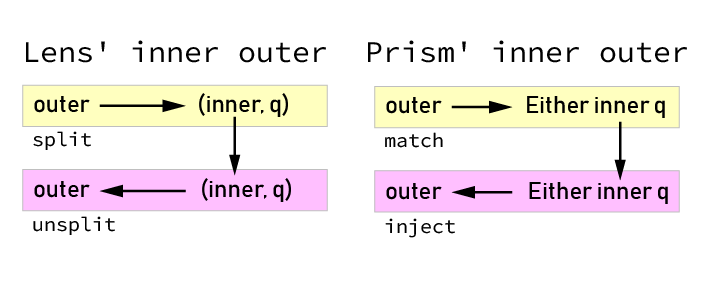
\includegraphics{/img/entries/lenses-and-prisms/lensprism1.png}
\caption{\texttt{Lens\textquotesingle{}\ inner\ outer} and
\texttt{Prism\textquotesingle{}\ inner\ outer} isomorphisms}
\end{figure}

Note how it is kind of complicated to talk about specific parts. If I say ``the
value of type \texttt{inner}'', do I mean the value ``before'' we use the lens,
or ``after'' we use the lens? There are two \texttt{inner}-typed values in our
picture.

A ``Lens family'' is a trick we can do to make talking about things easier. We
use the same lenses, but we \emph{re-label} the ``before'' and ``after'' (input
and output) with different type variables, like so:

\begin{figure}
\centering
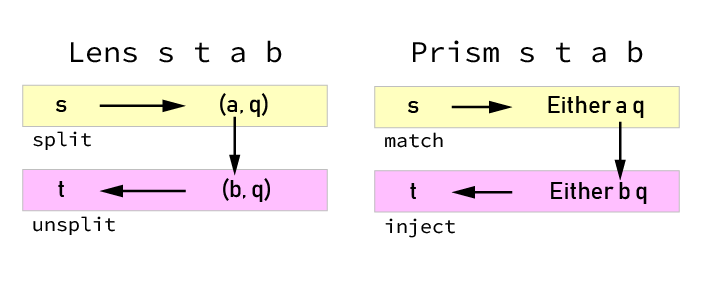
\includegraphics{/img/entries/lenses-and-prisms/lensprism2.png}
\caption{\texttt{Lens\ s\ t\ a\ b} and \texttt{Prism\ s\ t\ a\ b} isomorphisms,
as a lens family}
\end{figure}

Essentially, we're just deciding to give the inputs and outputs different type
variables. The main thing this helps is with is giving us the ability to
distinguish inputs from outputs when we talk about these things.

For example, before, with \texttt{Lens\textquotesingle{}\ outer\ inner}, if I
say ``the \texttt{outer}'', you won't know if I mean the \texttt{outer}
``before'' we use the lens, or the \texttt{outer} \emph{after} we use the lens.
However, with \texttt{Lens\ s\ t\ a\ b}, if I say ``the \texttt{s}'', you know
that I just mean ``the \texttt{outer} \emph{before} we use the lens'', and if I
say ``the \texttt{t}'', you know that I mean ``the \texttt{outer} \emph{after}
we use the lens''. The profunctor optics version of lens becomes
\texttt{Lens\ s\ t\ a\ b\ =\ p\ a\ b\ -\textgreater{}\ p\ s\ t}.

\texttt{Lens\ s\ t\ a\ b} (which is a version of
\texttt{Lens\textquotesingle{}\ outer\ inner} where we relabel the type
variables of the inputs and outputs) is called a
\href{http://comonad.com/reader/2012/mirrored-lenses/}{lens family}. Be careful
to never call it a ``polymorphic lens''. It is just a normal lens where we
re-label the type variables of all of the involved pieces to aid in our
discourse. It is often also called a ``type-changing lens''.

\begin{Shaded}
\begin{Highlighting}[]
\KeywordTok{data} \DataTypeTok{Lens}\NormalTok{ s t a b }\OtherTok{=} \KeywordTok{forall}\NormalTok{ q}\OperatorTok{.} \DataTypeTok{Lens}
\NormalTok{    \{}\OtherTok{ split   ::}\NormalTok{ s }\OtherTok{{-}>}\NormalTok{ (a, q)        }\CommentTok{{-}{-} before (with s and a)}
\NormalTok{    ,}\OtherTok{ unsplit ::}\NormalTok{ (b, q) }\OtherTok{{-}>}\NormalTok{ t        }\CommentTok{{-}{-} after  (with t and b)}
\NormalTok{    \}}

\OtherTok{view ::} \DataTypeTok{Lens}\NormalTok{ s t a b }\OtherTok{{-}>}\NormalTok{ (s }\OtherTok{{-}>}\NormalTok{ a)}
\OtherTok{set  ::} \DataTypeTok{Lens}\NormalTok{ s t a b }\OtherTok{{-}>}\NormalTok{ (b }\OtherTok{{-}>}\NormalTok{ s }\OtherTok{{-}>}\NormalTok{ t)}

\KeywordTok{data} \DataTypeTok{Prism}\NormalTok{ s t a b }\OtherTok{=} \KeywordTok{forall}\NormalTok{ q}\OperatorTok{.} \DataTypeTok{Prism}
\NormalTok{    \{}\OtherTok{ match  ::}\NormalTok{ s }\OtherTok{{-}>} \DataTypeTok{Either}\NormalTok{ a q     }\CommentTok{{-}{-} before (with s and a)}
\NormalTok{    ,}\OtherTok{ inject ::} \DataTypeTok{Either}\NormalTok{ b q }\OtherTok{{-}>}\NormalTok{ t     }\CommentTok{{-}{-} after  (with t and b)}
\NormalTok{    \}}

\OtherTok{matching ::} \DataTypeTok{Prism}\NormalTok{ s t a b }\OtherTok{{-}>}\NormalTok{ (s }\OtherTok{{-}>} \DataTypeTok{Either}\NormalTok{ t a)}
\OtherTok{review   ::} \DataTypeTok{Prism}\NormalTok{ s t a b }\OtherTok{{-}>}\NormalTok{ (b }\OtherTok{{-}>}\NormalTok{ t)}
\end{Highlighting}
\end{Shaded}

We still require \texttt{unsplit\ .\ split\ =\ id},
\texttt{split\ .\ unsplit\ =\ id}, \texttt{inject\ .\ match\ =\ id}, and
\texttt{match\ .\ inject\ =\ id}. They're all still \emph{isomorphisms}. We're
just \emph{relabeling our type variables} here to let us be more expressive with
how we talk about all of the moving parts.

Lens families can also be used to implement ``type changing lenses'' where
tweaking the inner type can cause the outer type to also change appropriately.
But \texttt{s}, \texttt{t}, \texttt{a}, and \texttt{b} can't just be whatever
you want. They have to be picked so that \texttt{unsplit\ .\ split} and
\texttt{inject\ .\ match} can typecheck.

\hypertarget{abstract-factors-and-addends}{%
\subsection{Abstract Factors and Addends}\label{abstract-factors-and-addends}}

In practice, the \texttt{q} to factor out your type into (in the
\texttt{s\ \textless{}\textasciitilde{}\textgreater{}\ (a,\ q)} and
\texttt{s\ \textless{}\textasciitilde{}\textgreater{}\ Either\ a\ q}) might not
be an actual ``concrete'' type. In most cases, it's alright to treat it as a
theoretical ``abstract'' type that follows the behavior you want given a
restricted interface. This is ``safe'' because, if you notice, none of the
methods in the lens or prism APIs (\texttt{view}, \texttt{set},
\texttt{preview}, \texttt{review}) ever let an external user directly manipulate
a value of type \texttt{q}.

For example, the
\texttt{only\ \textquotesingle{}a\textquotesingle{}\ ::\ Prism\textquotesingle{}\ Char\ ()}
prism matches only on \texttt{\textquotesingle{}a\textquotesingle{}}, and it is
the sum of \texttt{Char} and a theoretical abstract \texttt{Char} type that
excludes \texttt{\textquotesingle{}a\textquotesingle{}}.

To formalize this, sometimes we can say that only ``one direction'' of the
isomorphism has to be strictly true in practice. If we only enforce that the
round-trip of \texttt{unsplit\ .\ split\ =\ id} and
\texttt{inject\ .\ match\ =\ id}, this enforces the ``spirit'' of the hidden
abstract type.

For example, our ``\texttt{only\ \textquotesingle{}a\textquotesingle{}}'' can be
witnessed by:

\begin{Shaded}
\begin{Highlighting}[]
\CommentTok{{-}{-} source: https://github.com/mstksg/inCode/tree/master/code{-}samples/misc/lenses{-}and{-}prisms.hs\#L206{-}L350}

\KeywordTok{type} \DataTypeTok{CharButNotA} \OtherTok{=} \DataTypeTok{Char}

\OtherTok{onlyA ::} \DataTypeTok{Prism\textquotesingle{}} \DataTypeTok{Char}\NormalTok{ ()}
\NormalTok{onlyA }\OtherTok{=} \DataTypeTok{Prism\textquotesingle{}}
\NormalTok{    \{ match  }\OtherTok{=}\NormalTok{ \textbackslash{}}\KeywordTok{case}
        \CharTok{\textquotesingle{}a\textquotesingle{}} \OtherTok{{-}>} \DataTypeTok{Left}\NormalTok{ ()}
\NormalTok{        x   }\OtherTok{{-}>} \DataTypeTok{Right}\NormalTok{ (}\OtherTok{x ::} \DataTypeTok{CharButNotA}\NormalTok{)}
\NormalTok{    , inject }\OtherTok{=}\NormalTok{ \textbackslash{}}\KeywordTok{case}
        \DataTypeTok{Left}\NormalTok{  \_ }\OtherTok{{-}>} \CharTok{\textquotesingle{}a\textquotesingle{}}
        \DataTypeTok{Right}\NormalTok{ x }\OtherTok{{-}>}\NormalTok{ x        }\CommentTok{{-}{-} Right contains a CharButNotA}
\NormalTok{    \}}
\end{Highlighting}
\end{Shaded}

This passes \texttt{inject\ .\ match\ =\ id}, but not
\texttt{match\ .\ inject\ =\ id} if we pass in the ``illegal'' value
\texttt{Right\ \textquotesingle{}a\textquotesingle{}}.

For an example of a lens where this abstract type perspective is useful, there
is the \texttt{contains\ \textquotesingle{}a\textquotesingle{}} lens for sets:

\begin{Shaded}
\begin{Highlighting}[]
\CommentTok{{-}{-} import qualified Data.Set as S}

\NormalTok{contains }\CharTok{\textquotesingle{}a\textquotesingle{}}\OtherTok{ ::} \DataTypeTok{Lens\textquotesingle{}}\NormalTok{ (}\DataTypeTok{S.Set} \DataTypeTok{Char}\NormalTok{) }\DataTypeTok{Bool}

\CommentTok{{-}{-} check if a set contains an element}
\NormalTok{view (contains }\CharTok{\textquotesingle{}a\textquotesingle{}}\NormalTok{)}\OtherTok{ ::} \DataTypeTok{S.Set} \DataTypeTok{Char} \OtherTok{{-}>} \DataTypeTok{Bool}

\CommentTok{{-}{-} force a set to contain or not contain \textquotesingle{}a\textquotesingle{}}
\NormalTok{set (contains }\CharTok{\textquotesingle{}a\textquotesingle{}}\NormalTok{)}\OtherTok{ ::} \DataTypeTok{Bool} \OtherTok{{-}>} \DataTypeTok{S.Set} \DataTypeTok{Char} \OtherTok{{-}>} \DataTypeTok{S.Set} \DataTypeTok{Char}

\CommentTok{{-}{-} toggle membership in a set}
\NormalTok{over (contains }\CharTok{\textquotesingle{}a\textquotesingle{}}\NormalTok{)}\OtherTok{ not ::} \DataTypeTok{S.Set} \DataTypeTok{Char} \OtherTok{{-}>} \DataTypeTok{S.Set} \DataTypeTok{Char}
\end{Highlighting}
\end{Shaded}

\texttt{contains\ \textquotesingle{}a\textquotesingle{}} is a lens into a
\texttt{Bool} from a \texttt{S.Set}, where the \texttt{Bool} indicates if the
set ``contains'' \texttt{a} or not. What product does this represent?

Well, essentially,
\texttt{Set\ Char\ \textless{}\textasciitilde{}\textgreater{}\ (Bool,\ Set\ CharButNotA)}.
It's an abstract product betweein ``the set contains
\texttt{\textquotesingle{}a\textquotesingle{}} or not'' and a set that could not
possibly contain \texttt{\textquotesingle{}a\textquotesingle{}}:

\begin{Shaded}
\begin{Highlighting}[]
\CommentTok{{-}{-} source: https://github.com/mstksg/inCode/tree/master/code{-}samples/misc/lenses{-}and{-}prisms.hs\#L206{-}L217}

\KeywordTok{type} \DataTypeTok{CharButNotA} \OtherTok{=} \DataTypeTok{Char}

\OtherTok{containsA ::} \DataTypeTok{Lens\textquotesingle{}}\NormalTok{ (}\DataTypeTok{S.Set} \DataTypeTok{Char}\NormalTok{) }\DataTypeTok{Bool}
\NormalTok{containsA }\OtherTok{=} \DataTypeTok{Lens\textquotesingle{}}
\NormalTok{    \{ split   }\OtherTok{=}\NormalTok{ \textbackslash{}s }\OtherTok{{-}>}
\NormalTok{        ( }\CharTok{\textquotesingle{}a\textquotesingle{}} \OtherTok{\textasciigrave{}S.member\textasciigrave{}}\NormalTok{ s}
\NormalTok{        , }\CharTok{\textquotesingle{}a\textquotesingle{}} \OtherTok{\textasciigrave{}S.delete\textasciigrave{} s      ::} \DataTypeTok{S.Set} \DataTypeTok{CharButNotA}
\NormalTok{        )}
\NormalTok{    , unsplit }\OtherTok{=}\NormalTok{ \textbackslash{}}\KeywordTok{case}
\NormalTok{        (}\DataTypeTok{False}\NormalTok{, s) }\OtherTok{{-}>}\NormalTok{ s}
\NormalTok{        (}\DataTypeTok{True}\NormalTok{ , s) }\OtherTok{{-}>} \CharTok{\textquotesingle{}a\textquotesingle{}} \OtherTok{\textasciigrave{}S.insert\textasciigrave{}}\NormalTok{ (}\OtherTok{s ::} \DataTypeTok{S.Set} \DataTypeTok{CharButNotA}\NormalTok{)}
\NormalTok{    \}}
\end{Highlighting}
\end{Shaded}

Again, only \texttt{unsplit\ .\ split\ =\ id} is technically true.
\texttt{split\ .\ unsplit\ =\ id} will fail if the input set contains
\texttt{\textquotesingle{}a\textquotesingle{}}.

\hypertarget{exercises}{%
\subsection{Exercises}\label{exercises}}

To help solidify your understanding on this perspective, here are some
exercises! Most of them are conceptual and open-ended.

\begin{itemize}
\item
  We discussed the conditions where a type \texttt{a} can be expressed as a sum
  involving \texttt{()} and you can have a
  \texttt{Prism\textquotesingle{}\ a\ ()}.

  Under what conditions can you express a type \texttt{a} as a \emph{product}
  involving \texttt{Void}, and you can have a
  \texttt{Lens\textquotesingle{}\ a\ Void}? (Hint: use the algebra!) What would
  this lens do (what are \texttt{view}, \texttt{set}, and \texttt{over})?
\item
  We discussed the conditions where a type \texttt{a} can be expressed as a
  product involving \texttt{()} and you can have
  \texttt{Lens\textquotesingle{}\ a\ ()}.

  Under what conditions can you express a type \texttt{a} as a product involving
  \texttt{Bool}
  (\texttt{a\ \textless{}\textasciitilde{}\textgreater{}\ (Bool,\ q)}), and you
  can have a \texttt{Lens\textquotesingle{}\ a\ Bool}? (Hint: use the algebra!)
  What would this lens do (what are \texttt{view}, \texttt{set}, and
  \texttt{over})? And what about the \texttt{Lens\textquotesingle{}\ a\ q}?
\item
  We found that by interpreting \texttt{Either\ a\ a} as a product
  \texttt{(Bool,\ a)} gives us two interesting lenses:

\begin{Shaded}
\begin{Highlighting}[]
\OtherTok{leftOrRight ::} \DataTypeTok{Lens\textquotesingle{}}\NormalTok{ (}\DataTypeTok{Either}\NormalTok{ a a) }\DataTypeTok{Bool}
\OtherTok{theContents ::} \DataTypeTok{Lens\textquotesingle{}}\NormalTok{ (}\DataTypeTok{Either}\NormalTok{ a a) a}
\end{Highlighting}
\end{Shaded}

  We concluded that the first lens lets us flip between \texttt{Left} and
  \texttt{Right} or check if a value was \texttt{Left} or \texttt{Right}, and
  that the second lens gets into the contents regardless of leftness or
  rightness.

  However, there's a flip side, as well. \texttt{(Bool,\ a)} can be expressed as
  a \emph{sum} between \texttt{a} and itself, \texttt{Either\ a\ a}. This gives
  us two prisms:

\begin{Shaded}
\begin{Highlighting}[]
\CommentTok{{-}{-} source: https://github.com/mstksg/inCode/tree/master/code{-}samples/misc/lenses{-}and{-}prisms.hs\#L59{-}L69}

\OtherTok{mysteryPrism1 ::} \DataTypeTok{Prism\textquotesingle{}}\NormalTok{ (}\DataTypeTok{Bool}\NormalTok{, a) a}

\OtherTok{mysteryPrism2 ::} \DataTypeTok{Prism\textquotesingle{}}\NormalTok{ (}\DataTypeTok{Bool}\NormalTok{, a) a}
\end{Highlighting}
\end{Shaded}

  What do these prisms do? What is \texttt{preview}, \texttt{review},
  \texttt{over} for them?
\item
  Alright, now time to write code. Another ``interesting'' product is the fact
  that \texttt{Bool\ -\textgreater{}\ a} is isomorphic to \texttt{(a,\ a)}. That
  is, \texttt{Bool\ -\textgreater{}\ a} is a product between \texttt{a} and
  itself.

  Can you write the corresponding two
  \texttt{Lens\textquotesingle{}\ (Bool\ -\textgreater{}\ a)\ a}s? And, what do
  they mean? (what are \texttt{view}, \texttt{set}, \texttt{over} for those
  lenses?)
  \href{https://github.com/mstksg/inCode/tree/master/code-samples/misc/lenses-and-prisms.hs\#L43-L55}{Solutions
  online}
\item
  Can you write combinators to ``compose'' lenses and prisms? Is it even
  possible?

\begin{Shaded}
\begin{Highlighting}[]
\CommentTok{{-}{-} source: https://github.com/mstksg/inCode/tree/master/code{-}samples/misc/lenses{-}and{-}prisms.hs\#L81{-}L107}

\KeywordTok{data} \DataTypeTok{Lens\textquotesingle{}}\NormalTok{ s a }\OtherTok{=} \KeywordTok{forall}\NormalTok{ q}\OperatorTok{.} \DataTypeTok{Lens\textquotesingle{}}
\NormalTok{    \{}\OtherTok{ split   ::}\NormalTok{ s }\OtherTok{{-}>}\NormalTok{ (a, q)}
\NormalTok{    ,}\OtherTok{ unsplit ::}\NormalTok{ (a, q) }\OtherTok{{-}>}\NormalTok{ s}
\NormalTok{    \}}

\OtherTok{(.\&.) ::} \DataTypeTok{Lens\textquotesingle{}}\NormalTok{ a b}
      \OtherTok{{-}>} \DataTypeTok{Lens\textquotesingle{}}\NormalTok{ b c}
      \OtherTok{{-}>} \DataTypeTok{Lens\textquotesingle{}}\NormalTok{ a c}

\KeywordTok{data} \DataTypeTok{Prism\textquotesingle{}}\NormalTok{ s a }\OtherTok{=} \KeywordTok{forall}\NormalTok{ q}\OperatorTok{.} \DataTypeTok{Prism\textquotesingle{}}
\NormalTok{    \{}\OtherTok{ match  ::}\NormalTok{ s }\OtherTok{{-}>} \DataTypeTok{Either}\NormalTok{ a q}
\NormalTok{    ,}\OtherTok{ inject ::} \DataTypeTok{Either}\NormalTok{ a q }\OtherTok{{-}>}\NormalTok{ s}
\NormalTok{    \}}

\OtherTok{(.|.) ::} \DataTypeTok{Prism\textquotesingle{}}\NormalTok{ a b}
      \OtherTok{{-}>} \DataTypeTok{Prism\textquotesingle{}}\NormalTok{ b c}
      \OtherTok{{-}>} \DataTypeTok{Prism\textquotesingle{}}\NormalTok{ a c}
\end{Highlighting}
\end{Shaded}

  Roughtly speaking, composition of lenses or prisms are meant to ``successively
  zoom in'' to deeper and deeper parts of an initial structure.

  A note for you if you try this --- because the \texttt{q} type is existential,
  you can't use \texttt{split}, \texttt{unsplit}, \texttt{match}, or
  \texttt{inject} as record accessors, and you need to either pattern match or
  use \emph{-XRecordWildcards}.

  These implementations are pretty hairy (solutions
  \href{https://github.com/mstksg/inCode/tree/master/code-samples/misc/lenses-and-prisms.hs\#L81-L118}{online
  here}), and it's a sort of testament as to why we don't use this actual
  implementation in practice. In fact, for profunctor optics, we just have:

\begin{Shaded}
\begin{Highlighting}[]
\NormalTok{(}\OperatorTok{.\&.}\NormalTok{) }\OtherTok{=}\NormalTok{ (}\OperatorTok{.}\NormalTok{)}
\NormalTok{(}\OperatorTok{.|.}\NormalTok{) }\OtherTok{=}\NormalTok{ (}\OperatorTok{.}\NormalTok{)}
\end{Highlighting}
\end{Shaded}

  Using \texttt{(.)} from \texttt{Prelude}. Definitely much simpler! (And it's
  one main reason why they're among the most popular representation)
\end{itemize}

\hypertarget{special-thanks}{%
\section{Special Thanks}\label{special-thanks}}

I am very humbled to be supported by an amazing community, who make it possible
for me to devote time to researching and writing these posts. Very special
thanks to my supporter at the ``Amazing'' level on
\href{https://www.patreon.com/justinle/overview}{patreon}, Sam Stites! :)

\hypertarget{signoff}{%
\section{Signoff}\label{signoff}}

Hi, thanks for reading! You can reach me via email at
\href{mailto:justin@jle.im}{\nolinkurl{justin@jle.im}}, or at twitter at
\href{https://twitter.com/mstk}{@mstk}! This post and all others are published
under the \href{https://creativecommons.org/licenses/by-nc-nd/3.0/}{CC-BY-NC-ND
3.0} license. Corrections and edits via pull request are welcome and encouraged
at \href{https://github.com/mstksg/inCode}{the source repository}.

If you feel inclined, or this post was particularly helpful for you, why not
consider \href{https://www.patreon.com/justinle/overview}{supporting me on
Patreon}, or a \href{bitcoin:3D7rmAYgbDnp4gp4rf22THsGt74fNucPDU}{BTC donation}?
:)

\end{document}
